\documentclass[11pt]{article}

\usepackage[margin=1in]{geometry}
\usepackage{amsmath, amssymb, amsfonts}
\usepackage{bm}
\usepackage{graphicx}
\usepackage{enumitem}
\usepackage{tikz}
\usetikzlibrary{calc,decorations.pathmorphing,patterns}
\usepackage[most]{tcolorbox}
\usepackage{hyperref}
\usepackage{booktabs}

\title{Ice Rheology Part 2: Elasticity and Viscoelasticity}
\author{Brent Minchew \\Caltech Ge 193, Spring 2026}
\date{}

\begin{document}

\maketitle

%===================================================================
% Topics Covered
%===================================================================
\section*{Topics Covered}

\begin{itemize}
  \item Linear elasticity and Hooke's law for isotropic materials
  \item Elastic moduli and wave speeds in ice
  \item Maxwell viscoelasticity and the relaxation time
  \item Elastic flexure of floating ice
  \item Examples: grounding zone tidal flexure, j\"{o}kulhlaups, and supraglacial lake drainage
\end{itemize}

\noindent\textbf{Primary reference:} Cuffey \& Paterson, \textit{Physics of Glaciers}, 4th ed., Chapters~3 and~10; Petrenko \& Whitworth, \textit{Physics of Ice}, Chapter~4.

%===================================================================
% SECTION 1 -- Introduction and Motivation
%===================================================================
\section{Introduction and Motivation}
\label{sec:introduction}

In the preceding lectures on ice rheology, we treated ice as a viscous fluid where stress determines the rate of deformation, and there is no memory of past states (or strain).  Glen's flow law and the composite flow law of \cite{GoldsbyKohlstedt2001} describe the long-term, steady-state creep behavior of ice under sustained loading.  This viscous description is appropriate for processes that unfold over timescales much longer than the material's relaxation time, a material property we define later that varies between hours and days in terrestrial glaciers.

\medskip
\noindent Many important glaciological processes, however, occur on timescales short enough that ice might behave elastically.  Tidal loading at grounding zones flexes ice shelves with periods of hours.  J\"{o}kulhlaups drain subglacial lakes over hours to days.  Supraglacial lakes load ice shelves and can drain catastrophically in minutes.  On these timescales, ice can deform like an elastic solid where the Cauchy stress is proportional to strain (symmetric component of the gradient of displacement). In an elastic material, deformation is recoverable when the load is removed.

\medskip
\noindent The goal of this lecture is to develop the elastic and viscoelastic constitutive relations for ice, building on the viscous framework established earlier.  We begin with linear elasticity---the simplest constitutive model for a solid material---and derive Hooke's law.  We then introduce the Maxwell viscoelastic model, which combines elastic and viscous behavior in a single framework and provides a natural transition between the short-timescale elastic response and the long-timescale viscous flow we have already studied.  Worked examples illustrate the application of these ideas to grounding zone flexure, j\"{o}kulhlaups, and ice-shelf hydrofracture.

\medskip
\noindent Two appendices derive Hooke's law and the heat equation from the first law of thermodynamics, showing how elasticity (the reversible storage of energy through molecular displacement) and heat conduction (the irreversible transport of energy through molecular vibration) arise from the same fundamental energy balance.

\medskip
\noindent\textbf{Plan for this lecture.}  We review linear elasticity and Hooke's law (\S\ref{sec:elasticity}), present the elastic properties of ice (\S\ref{sec:elastic_moduli}), develop the elastic flexure equation for thin plates (\S\ref{sec:flexure}), introduce Maxwell viscoelasticity (\S\ref{sec:maxwell}), and work through three glaciological examples (\S\ref{sec:worked_examples}).  Appendix~\ref{app:hookes_law} derives Hooke's law from the first law of thermodynamics; Appendix~\ref{app:heat_equation} derives the standard heat equation; Appendix~\ref{app:generalized_heat} derives the generalized heat equation that includes viscous dissipation and recrystallization; and Appendix~\ref{app:flexure_derivation} derives the thin plate flexure equation from the force balance on a plate element.

%===================================================================
% SECTION 2 -- Linear Elasticity
%===================================================================
\section{Linear Elasticity}
\label{sec:elasticity}

\subsection{Stress and Infinitesimal Strain}
\label{sec:strain}

In the viscous framework developed in earlier lectures, the constitutive relation links deviatoric stress to the \textit{rate} of deformation: $\dot{\varepsilon}_{ij} = f(\tau_{ij})$.  In an elastic solid, the constitutive relation links Cauchy stress to the deformation itself: $\sigma_{ij} = g(\varepsilon_{ij})$.

\medskip
\noindent The Cauchy stress tensor $\sigma_{ij}$ and its decomposition into pressure and deviatoric parts,
\begin{equation}
  \sigma_{ij} = -p\,\delta_{ij} + \tau_{ij}, \qquad p = -\tfrac{1}{3}\sigma_{kk}, \qquad \tau_{kk} = 0,
  \label{eq:stress_decomposition}
\end{equation}
are the same as in the viscous theory.  What changes is the kinematic quantity to which stress is related.

\medskip
\noindent For small deformations, we define the \textbf{infinitesimal strain tensor}:
\begin{equation}
  \varepsilon_{ij} = \frac{1}{2}\!\left(\frac{\partial s_i}{\partial x_j} + \frac{\partial s_j}{\partial x_i}\right),
  \label{eq:strain_tensor}
\end{equation}
where $s_i$ is the displacement of a material point from its reference position.  We reserve $u_i$ for velocity, as in the viscous theory, so that $u_i = \dot{s}_i$ and the strain rate is $\dot{\varepsilon}_{ij} = \frac{1}{2}(\partial u_i / \partial x_j + \partial u_j / \partial x_i)$.  The two frameworks are connected by a time derivative: $\dot{\varepsilon}_{ij}$ is the \emph{instantaneous} rate of change of $\varepsilon_{ij}$. Strain $\varepsilon_{ij}$ is always defined relative to the reference (zero-stress) state, whereas strain rate is the instantaneous rate of change of strain.  Because strain is a state variable, it evolves over time and not necessarily at the same rate nor even monotonically, a critically important fact to remember. Much confusion can arise from forgetting that strain is relative to the reference state. 

\medskip
\noindent The ``small deformation'' assumption means $|\varepsilon_{ij}| \ll 1$, allowing us to drop higher-order terms in the full expansion and retain only the linear terms --- hence, \emph{linear} elasticity. In glaciology, elastic strains are tiny: a stress of $\tau_e = 0.1$~MPa produces an elastic strain of order $\varepsilon \sim \tau_e / \mu \sim 10^5 / 3.5 \times 10^9 \approx 3 \times 10^{-5}$.  The small-strain approximation is therefore excellent for the elastic response of ice. (Pedantic: Linear elasticity strictly requires both small strains and a stress--strain relation that is linear and rate-independent.  Ice exhibits a weak frequency dependence of its elastic moduli---a form of anelasticity---which means the moduli measured at seismic frequencies differ slightly from those at tidal frequencies.  This is a departure from ideal linear elasticity, though it is a small effect at glaciological stress levels.)

\subsection{Hooke's Law}
\label{sec:hookes_law}

For a linear elastic material, stress is a linear function of strain.  The most general linear relation between two second-order tensors is
\begin{equation}
  \boxed{\sigma_{ij} = C_{ijkl}\,\varepsilon_{kl},}
  \label{eq:hookes_law_general}
\end{equation}
where $C_{ijkl}$ is the \textbf{fourth-order elastic stiffness tensor}.  This is Hooke's law in its most general form.  The stiffness tensor has $3^4 = 81$ components, but symmetry reduces the number of independent components:
\begin{itemize}
  \item Symmetry of the stress tensor ($\sigma_{ij} = \sigma_{ji}$) requires $C_{ijkl} = C_{jikl}$, reducing 81 to 54.
  \item Symmetry of the strain tensor ($\varepsilon_{kl} = \varepsilon_{lk}$) requires $C_{ijkl} = C_{ijlk}$, reducing 54 to 36.
  \item The existence of a strain energy function (Appendix~\ref{app:hookes_law}) requires $C_{ijkl} = C_{klij}$, reducing 36 to 21.
\end{itemize}
For a fully anisotropic crystal, 21 independent elastic constants are needed.  Ice Ih has hexagonal symmetry, which reduces this to 5 independent constants.  For polycrystalline ice with randomly oriented grains---the isotropic approximation---only 2 independent constants remain.

\subsection{Isotropic Hooke's Law}
\label{sec:isotropic}

For an \textbf{isotropic} material, the stiffness tensor must be invariant under all rotations.  The most general fourth-order isotropic tensor with the required symmetries is
\begin{equation}
  C_{ijkl} = \lambda\,\delta_{ij}\,\delta_{kl} + \mu\!\left(\delta_{ik}\,\delta_{jl} + \delta_{il}\,\delta_{jk}\right),
  \label{eq:isotropic_stiffness}
\end{equation}
where $\lambda$ and $\mu$ are the \textbf{Lam\'{e} parameters}.  Substituting into equation~\eqref{eq:hookes_law_general}:
\begin{equation}
  \boxed{\sigma_{ij} = \lambda\,\varepsilon_{kk}\,\delta_{ij} + 2\mu\,\varepsilon_{ij}.}
  \label{eq:hookes_law_isotropic}
\end{equation}
This is Hooke's law for an isotropic solid.  The parameter $\mu$ is the \textbf{shear modulus} (also denoted $G$), which relates shear stress to shear strain.  The parameter $\lambda$ is the \textbf{first Lam\'{e} parameter}, which does not have as clean a physical interpretation on its own but appears naturally in the isotropic form.

\medskip
\noindent The volumetric and deviatoric parts of Hooke's law separate cleanly.  Taking the trace of equation~\eqref{eq:hookes_law_isotropic}:
\begin{equation}
  \sigma_{kk} = (3\lambda + 2\mu)\,\varepsilon_{kk},
  \label{eq:volumetric}
\end{equation}
so that $p = -\frac{1}{3}(3\lambda + 2\mu)\,\varepsilon_{kk}$.  The \textbf{bulk modulus} $K = \lambda + \frac{2}{3}\mu$ controls the volumetric response.  The deviatoric part is
\begin{equation}
  \tau_{ij} = 2\mu\,e_{ij},
  \label{eq:deviatoric_hooke}
\end{equation}
where $e_{ij} = \varepsilon_{ij} - \frac{1}{3}\varepsilon_{kk}\,\delta_{ij}$ is the deviatoric strain.  The shear modulus $\mu$ alone controls the deviatoric (shape-changing) response.

\medskip
\noindent\textbf{Physical meaning of the elastic moduli.}  Each modulus characterizes the material's resistance to a specific type of deformation (Figure~\ref{fig:elastic_moduli_cartoons}):
\begin{itemize}
  \item \textbf{Shear modulus} $\mu$ (also denoted $G$): the ratio of shear stress to shear strain.  Apply a shear stress $\tau_{xy}$ to a block of material; the block deforms into a parallelogram with shear strain $\varepsilon_{xy} = \tau_{xy}/(2\mu)$.  The shear modulus controls shape change at constant volume.

  \item \textbf{Young's modulus} $E$: the ratio of axial stress to axial strain in uniaxial tension (or compression).  Stretch a bar with stress $\sigma_{xx}$ along $x$ while leaving the lateral faces traction-free ($\sigma_{yy} = \sigma_{zz} = 0$); the axial strain is $\varepsilon_{xx} = \sigma_{xx}/E$.  Young's modulus characterizes the stiffness felt in a simple pull test.

  \item \textbf{Poisson's ratio} $\nu$: the ratio of lateral contraction to axial extension in uniaxial tension.  In the same pull test, the lateral strains are $\varepsilon_{yy} = \varepsilon_{zz} = -\nu\,\varepsilon_{xx}$.  A material with $\nu = 0.5$ is incompressible (no volume change); $\nu = 0$ means no lateral contraction.

  \item \textbf{Bulk modulus} $K$: the ratio of pressure to volumetric strain under uniform compression.  Apply a uniform pressure $p$ to all faces of a cube; the fractional volume change is $\varepsilon_{kk} = -p/K$.  The bulk modulus controls volume change at constant shape.
\end{itemize}

\begin{tcolorbox}[
  colback=blue!5,
  colframe=blue!50!black,
  title={\textbf{Key point: two independent moduli}}
]
An isotropic elastic solid is fully characterized by two independent elastic constants.  Common pairs include:
\begin{center}
\small
\begin{tabular}{ll}
\toprule
\textbf{Pair} & \textbf{Physical interpretation} \\
\midrule
$\lambda$, $\mu$ & Lam\'{e} parameters (natural in the tensor form) \\
$K$, $\mu$ & Bulk modulus (volumetric) and shear modulus (deviatoric) \\
$E$, $\nu$ & Young's modulus (uniaxial stiffness) and Poisson's ratio (lateral contraction) \\
\bottomrule
\end{tabular}
\end{center}
All pairs are equivalent; the choice is one of convenience.  The relations are:
\begin{equation}
  \lambda = K - \tfrac{2}{3}\mu = \frac{E\nu}{(1+\nu)(1-2\nu)}, \qquad \mu = \frac{E}{2(1+\nu)}, \qquad K = \frac{E}{3(1-2\nu)}.
  \label{eq:moduli_relations}
\end{equation}
\end{tcolorbox}

\begin{figure}[ht]
\centering
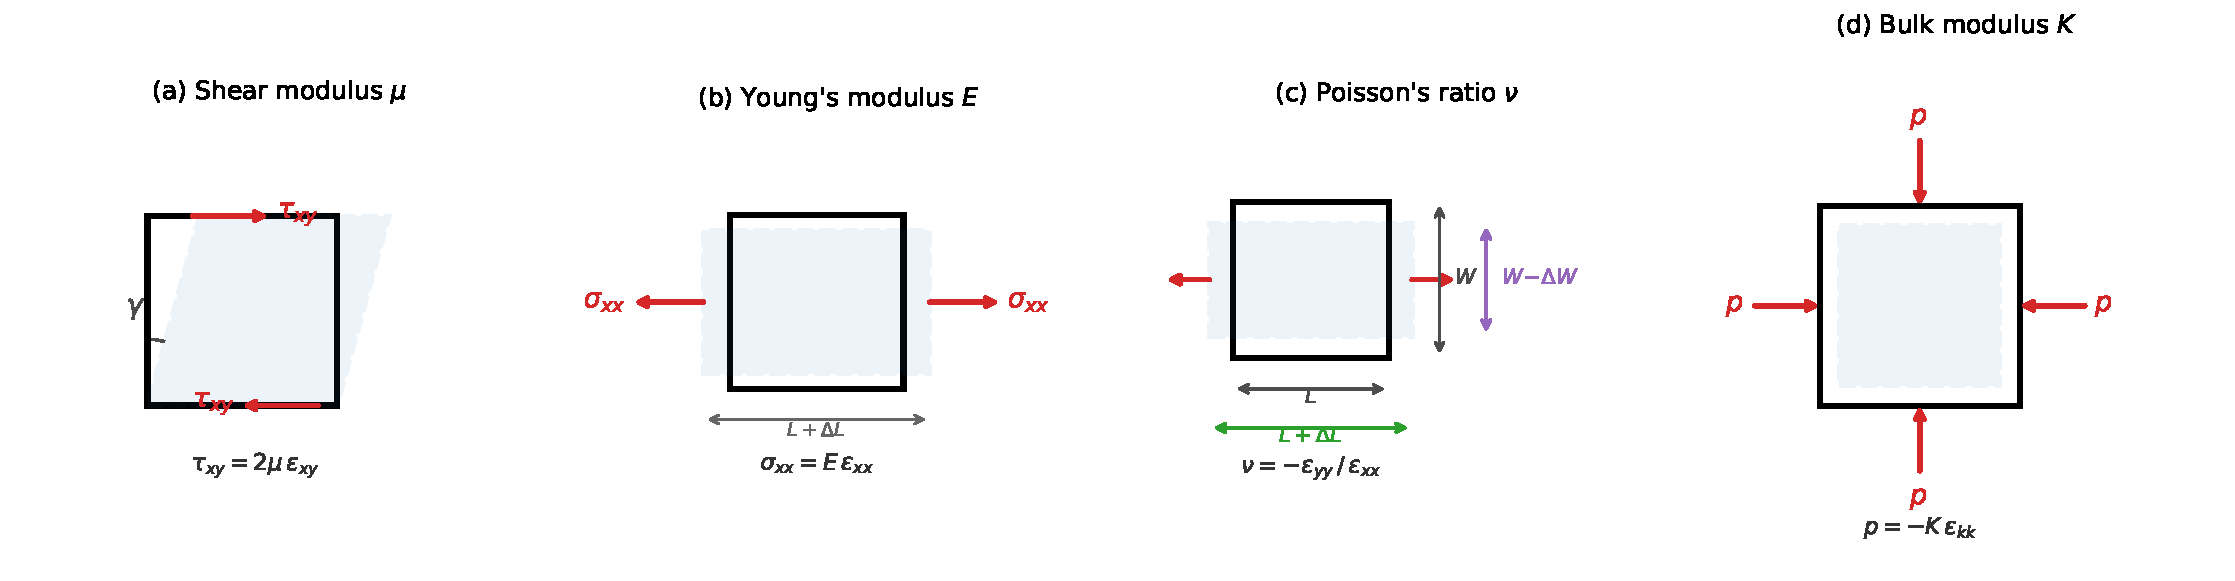
\includegraphics[width=\textwidth]{figures/fig06_elastic_moduli_cartoons.pdf}
\caption{Schematic illustrations of the four primary elastic moduli.  Solid rectangles show the undeformed reference state; dashed outlines show the deformed state.  (a)~Shear modulus $\mu$: shear stress produces angular distortion at constant volume.  (b)~Young's modulus $E$: uniaxial tension produces axial extension and lateral contraction.  (c)~Poisson's ratio $\nu$: the ratio of lateral contraction to axial extension in a uniaxial test.  (d)~Bulk modulus $K$: uniform pressure produces uniform volume change at constant shape.}
\label{fig:elastic_moduli_cartoons}
\end{figure}

%===================================================================
% SECTION 3 -- Elastic Moduli of Ice
%===================================================================
\section{Elastic Properties of Ice}
\label{sec:elastic_moduli}

\subsection{Measured Elastic Moduli}

The elastic moduli of polycrystalline ice Ih have been measured by a variety of techniques, including ultrasonic wave propagation, Brillouin spectroscopy, and mechanical testing.  The most precise values come from wave-speed measurements, which probe the high-frequency (truly elastic) response without contamination from viscous creep.  Table~\ref{tab:elastic_moduli} summarizes the isotropic elastic constants for polycrystalline ice near $-10$\textdegree C \cite{Gammonetal1983}.

\begin{table}[ht]
\centering
\caption{Isotropic elastic moduli of polycrystalline ice Ih at $-10$\textdegree C \cite{Gammonetal1983}.  Values are Hill averages of the five single-crystal elastic constants, which provide the best estimate of the isotropic elastic response of a polycrystal with randomly oriented grains.}
\label{tab:elastic_moduli}
\begin{tabular}{lcc}
\toprule
\textbf{Quantity} & \textbf{Symbol} & \textbf{Value} \\
\midrule
Young's modulus & $E$ & 9.33 GPa \\
Shear modulus & $\mu$ & 3.52 GPa \\
Bulk modulus & $K$ & 8.90 GPa \\
First Lam\'{e} parameter & $\lambda$ & 6.55 GPa \\
Poisson's ratio & $\nu$ & 0.325 \\
\bottomrule
\end{tabular}
\end{table}

\noindent Several features of these values are worth noting:
\begin{enumerate}
  \item \textbf{Ice is a stiff solid.}  The shear modulus of ice ($\mu = 3.5$~GPa) is about 25 times that of lead (0.14~GPa) and roughly 1/20 that of steel (80~GPa).  The elastic response of ice is well described by the theory of linear elasticity---there is no measurable nonlinearity at glaciological stress levels.

  \item \textbf{Poisson's ratio is close to 1/3.}  A Poisson's ratio $\nu = 0.325$ means that ice contracts laterally by about one-third of the amount it extends axially under uniaxial tension.  For comparison, $\nu = 0.5$ corresponds to an incompressible material (no volume change under any deformation), and $\nu = 0$ corresponds to a material that does not contract laterally at all (like cork).

  \item \textbf{Temperature dependence is weak.}  The elastic moduli increase by roughly 5\% between 0\textdegree C and $-40$\textdegree C \cite{Gammonetal1983}.  This is a minor effect compared to the strong temperature dependence of viscous creep (activation energies of 49--180~kJ\,mol$^{-1}$).  For most glaciological calculations, the elastic moduli can be treated as constants.

  \item \textbf{The shear modulus has a weak frequency dependence.}  The values in Table~\ref{tab:elastic_moduli} are measured at ultrasonic frequencies ($\sim$MHz) and represent the unrelaxed (instantaneous) elastic response.  At lower frequencies---tidal ($\sim 10^{-5}$~Hz) or seismic ($\sim$1--100~Hz)---the effective shear modulus is slightly lower because thermally activated processes at grain boundaries and lattice defects allow a small amount of anelastic relaxation on the timescale of each loading cycle.  Physically, this arises because grain boundaries in polycrystalline ice can slide viscously over short distances (grain boundary sliding) and dislocations can bow between pinning points, both of which accommodate a small additional strain that is recoverable but delayed.  At high frequencies, these relaxation mechanisms cannot keep pace with the loading and the material responds with the full lattice stiffness; at lower frequencies, the mechanisms contribute additional compliance.  The effect is small---the shear modulus decreases by roughly 5--10\% from MHz to tidal frequencies---but it means that the ``elastic modulus'' inferred from tidal flexure observations is systematically lower than the laboratory ultrasonic value, even before accounting for viscous creep (which further reduces the effective modulus through the viscoelastic mechanism described in \S\ref{sec:maxwell}).
\end{enumerate}

\subsection{Elastic Wave Speeds}
\label{sec:wave_speeds}

The elastic moduli determine the speeds of seismic waves in ice.  Substituting Hooke's law~\eqref{eq:hookes_law_isotropic} into Cauchy's equation of motion ($\sigma_{ij,j} + f_i = \rho\,\ddot{s}_i$, in the absence of body forces) yields the Navier--Cauchy equation:
\begin{equation}
  (\lambda + \mu)\,\frac{\partial^2 s_j}{\partial x_i \partial x_j} + \mu\,\frac{\partial^2 s_i}{\partial x_j \partial x_j} = \rho\,\frac{\partial^2 s_i}{\partial t^2}.
  \label{eq:navier_cauchy}
\end{equation}
This wave equation admits two types of plane-wave solutions:
\begin{itemize}
  \item \textbf{P-waves} (compressional): $v_p = \sqrt{(\lambda + 2\mu)/\rho} = \sqrt{(K + \frac{4}{3}\mu)/\rho}$,
  \item \textbf{S-waves} (shear): $v_s = \sqrt{\mu/\rho}$.
\end{itemize}
For ice ($\rho_i = 917$~kg\,m$^{-3}$):
\begin{equation}
  v_p = \sqrt{\frac{6550 + 2 \times 3520}{917} \times 10^6} \approx 3850 \text{ m\,s}^{-1}, \qquad v_s = \sqrt{\frac{3520 \times 10^6}{917}} \approx 1960 \text{ m\,s}^{-1}.
  \label{eq:wave_speeds}
\end{equation}
These values agree well with seismic observations in glaciers and ice sheets \cite{KohnenBentley1973}.  The P-wave speed in ice is notably higher than in water (1480~m\,s$^{-1}$) and lower than in most rocks (4000--7000~m\,s$^{-1}$).

%===================================================================
% SECTION 4 -- Elastic Flexure of Thin Plates
%===================================================================
\section{Elastic Flexure of Thin Plates}
\label{sec:flexure}

Many glaciological applications of elasticity involve the bending of ice shelves and glacier tongues---structures that are thin compared to their horizontal extent.  The theory of thin elastic plates provides an efficient framework for these problems.

\subsection{The Flexure Equation}
\label{sec:flexure_equation}

Consider a thin plate of thickness $h$ and flexural rigidity
\begin{equation}
  D = \frac{E\,h^3}{12(1-\nu^2)},
  \label{eq:flexural_rigidity}
\end{equation}
resting on or floating in a fluid of density $\rho_w$.  Let $w(x,y)$ denote the vertical deflection of the plate from its equilibrium position.  For small deflections ($|w| \ll h$), the governing equation is
\begin{equation}
  \boxed{D\,\nabla^4 w + \rho_w\,g\,w = q(x,y),}
  \label{eq:plate_flexure}
\end{equation}
where $\nabla^4 = \partial^4/\partial x^4 + 2\,\partial^4/(\partial x^2\,\partial y^2) + \partial^4/\partial y^4$ is the biharmonic operator, $\rho_w\,g\,w$ is the buoyancy restoring force per unit area (for a floating plate), and $q(x,y)$ is any applied load per unit area.  Appendix~\ref{app:flexure_derivation} derives this equation from the force and moment balance on a plate element.

\medskip
\noindent In one horizontal dimension (e.g., a beam or a plate that varies only in $x$):
\begin{equation}
  D\,\frac{d^4 w}{dx^4} + \rho_w\,g\,w = q(x).
  \label{eq:beam_flexure}
\end{equation}
The homogeneous solution (with $q = 0$) involves a characteristic length scale, the \textbf{flexural wavelength}:
\begin{equation}
  \boxed{\ell_f = \left(\frac{4D}{\rho_w\,g}\right)^{1/4} = \left(\frac{E\,h^3}{3(1-\nu^2)\,\rho_w\,g}\right)^{1/4}.}
  \label{eq:flexural_wavelength}
\end{equation}
The flexural wavelength sets the horizontal distance over which the plate adjusts from a loaded to an unloaded state.  Features much smaller than $\ell_f$ are supported by the plate's rigidity; features much larger than $\ell_f$ are in isostatic equilibrium with the underlying fluid.

\subsection{Flexural Wavelength of Ice Shelves}

For an ice shelf of thickness $h$, using $E = 9.33$~GPa, $\nu = 0.325$, and $\rho_w = 1025$~kg\,m$^{-3}$:
\begin{equation}
  \ell_f = \left(\frac{9.33 \times 10^9 \times h^3}{3 \times 0.894 \times 1025 \times 9.8}\right)^{1/4} = \left(\frac{9.33 \times 10^9}{2.70 \times 10^4}\right)^{1/4} h^{3/4} \approx 24.2\;h^{3/4},
  \label{eq:lf_ice}
\end{equation}
where $h$ is in meters and $\ell_f$ is in meters.  Representative values:

\begin{center}
\begin{tabular}{ccc}
\toprule
Ice thickness $h$ (m) & Flexural rigidity $D$ (N\,m) & Flexural wavelength $\ell_f$ (km) \\
\midrule
200 & $6.9 \times 10^{15}$ & 1.3 \\
500 & $1.1 \times 10^{17}$ & 2.6 \\
1000 & $8.7 \times 10^{17}$ & 4.3 \\
\bottomrule
\end{tabular}
\end{center}

\noindent The flexural wavelength is typically 1--5~km for Antarctic ice shelves.  This length scale appears repeatedly in our worked examples.

\subsection{Bending Stresses}
\label{sec:bending_stresses}

The bending of a thin plate produces normal stresses that vary linearly through the thickness:
\begin{equation}
  \sigma_{xx}(z) = -\frac{E\,z}{1-\nu^2}\left(\frac{\partial^2 w}{\partial x^2} + \nu\,\frac{\partial^2 w}{\partial y^2}\right),
  \label{eq:bending_stress}
\end{equation}
where $z$ is measured from the plate's neutral surface (midplane), with $z > 0$ upward.  The maximum tensile stress occurs at the surface farthest from the center of curvature.  For a plate deflecting downward ($w < 0$, concave upward), the maximum tensile stress is at the bottom surface ($z = -h/2$).  For a plate deflecting upward, the maximum tensile stress is at the top surface.

\medskip
\noindent In one horizontal dimension:
\begin{equation}
  \sigma_{xx}^{\text{max}} = \frac{E\,h}{2(1-\nu^2)}\left|\frac{d^2 w}{dx^2}\right| = \frac{6\,|M|}{h^2},
  \label{eq:max_bending_stress}
\end{equation}
where $M = -D\,d^2w/dx^2$ is the bending moment per unit width.

%===================================================================
% SECTION 5 -- Maxwell Viscoelasticity
%===================================================================
\section{Maxwell Viscoelasticity}
\label{sec:maxwell}

\subsection{The Maxwell Model}
\label{sec:maxwell_model}

The creep flow laws developed in the preceding lecture describe the long-timescale behavior of ice under sustained loading.  The elastic theory of \S\ref{sec:elasticity} describes the instantaneous response to a change in load.  To bridge these regimes, we need a constitutive model that includes both elastic and viscous behavior.  The simplest such model is the \textbf{Maxwell model}, which places an elastic element (spring) and a viscous element (dashpot) in series.

\begin{center}
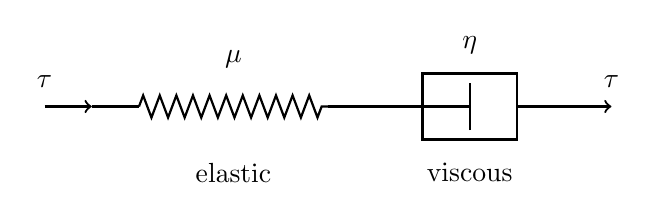
\begin{tikzpicture}[scale=1.2]
  % Spring
  \draw[thick] (0,0) -- (0.5,0);
  \draw[thick, decorate, decoration={zigzag, segment length=6, amplitude=4}] (0.5,0) -- (2.5,0);
  \draw[thick] (2.5,0) -- (3.0,0);
  \node[above] at (1.5,0.3) {$\mu$};
  % Dashpot
  \draw[thick] (3.0,0) -- (3.5,0);
  \draw[thick] (3.5,-0.35) rectangle (4.5,0.35);
  \draw[thick] (3.5,0) -- (4.0,0);
  \draw[thick, fill=gray!30] (4.0,-0.25) -- (4.0,0.25);
  \draw[thick] (4.5,0) -- (5.0,0);
  \node[above] at (4.0,0.45) {$\eta$};
  % Labels
  \node[below] at (1.5,-0.5) {elastic};
  \node[below] at (4.0,-0.5) {viscous};
  % Arrows
  \draw[thick, ->] (-0.5,0) -- (0,0);
  \draw[thick, ->] (5.0,0) -- (5.5,0);
  \node[above] at (-0.5,0.1) {$\tau$};
  \node[above] at (5.5,0.1) {$\tau$};
\end{tikzpicture}
\end{center}

\noindent In a series arrangement, both elements carry the same stress, and the total strain rate is the sum of the individual strain rates:
\begin{equation}
  \dot{\varepsilon}_{ij} = \dot{\varepsilon}_{ij}^{(\text{elastic})} + \dot{\varepsilon}_{ij}^{(\text{viscous})}.
  \label{eq:maxwell_decomposition}
\end{equation}
The elastic strain rate is the time derivative of the elastic constitutive relation~\eqref{eq:deviatoric_hooke}:
\begin{equation}
  \dot{\varepsilon}_{ij}^{(\text{elastic})} = \frac{1}{2\mu}\,\dot{\tau}_{ij}.
  \label{eq:elastic_rate}
\end{equation}
assuming incompressibility. The viscous strain rate is given by the creep flow law.  For Glen's law:
\begin{equation}
  \dot{\varepsilon}_{ij}^{(\text{viscous})} = A\,\tau_e^{\,n-1}\,\tau_{ij}.
  \label{eq:viscous_rate}
\end{equation}
Combining:
\begin{equation}
  \boxed{\dot{\varepsilon}_{ij} = \frac{1}{2\mu}\,\dot{\tau}_{ij} + A\,\tau_e^{\,n-1}\,\tau_{ij}.}
  \label{eq:maxwell_constitutive}
\end{equation}
This is the Maxwell viscoelastic constitutive equation for ice.  The first term describes the instantaneous elastic response to changes in stress; the second describes the ongoing viscous creep under sustained stress.

\medskip
\noindent Equation~\eqref{eq:maxwell_constitutive} is written for the deviatoric part of the stress--strain relation.  For the volumetric part, we assume a purely elastic response:
\begin{equation}
  \sigma_{kk} = 3K\,\varepsilon_{kk},
\end{equation}
because ice does not undergo viscous volume change (the creep mechanisms are isochoric).

\subsection{The Maxwell Relaxation Time}
\label{sec:maxwell_time}

The Maxwell model has a characteristic timescale, the \textbf{relaxation time}, that separates elastic-dominated from viscous-dominated behavior.  To find it, consider the 1D version of equation~\eqref{eq:maxwell_constitutive} and suppose the total strain is held fixed ($\dot{\varepsilon} = 0$) after an instantaneous loading.  Then
\begin{equation}
  \frac{1}{2\mu}\,\dot{\tau} + \frac{\tau}{2\eta} = 0,
  \label{eq:stress_relaxation_ode}
\end{equation}
where $\eta$ is the effective viscosity, related to Glen's law by $\eta = \tau_e / (2\dot{\varepsilon}_e) = 1/(2A\,\tau_e^{\,n-1})$.  For constant $\eta$ (i.e., Newtonian viscosity or linearization about a given stress), the solution is exponential decay:
\begin{equation}
  \tau(t) = \tau_0\,\exp\!\left(-t/t_M\right), \qquad t_M = \frac{\eta}{\mu}.
  \label{eq:stress_relaxation}
\end{equation}
The \textbf{Maxwell time} $t_M = \eta/\mu$ is the $e$-folding time for stress relaxation at constant strain.  It has a direct physical meaning: elastic stresses decay on a timescale $t_M$ as the viscous element takes up the deformation.

\medskip
\noindent For ice with Glen's law ($n = 3$), the effective viscosity $\eta = 1/(2A\,\tau_e^2)$ depends on the stress level, so the Maxwell time is also stress-dependent:
\begin{equation}
  \boxed{t_M = \frac{1}{2\mu\,A\,\tau_e^{\,n-1}}.}
  \label{eq:maxwell_time}
\end{equation}
The Maxwell time is short where ice is warm and highly stressed, and long where ice is cold and under low stress.  Table~\ref{tab:maxwell_times} gives representative values.

\begin{table}[ht]
\centering
\caption{Maxwell relaxation time $t_M$ for polycrystalline ice under different conditions, computed from equation~\eqref{eq:maxwell_time} using $\mu = 3.5$~GPa, $n = 3$, and values of $A$ from the Arrhenius relation with $Q = 60$~kJ\,mol$^{-1}$ (below 263~K) and $Q = 139$~kJ\,mol$^{-1}$ (above 263~K).}
\label{tab:maxwell_times}
\begin{tabular}{lcccl}
\toprule
\textbf{Setting} & $T$ (K) & $\tau_e$ (MPa) & $A$ (Pa$^{-3}$\,s$^{-1}$) & $t_M$ \\
\midrule
Warm shear margin & 270 & 0.2 & $2.0 \times 10^{-24}$ & 30 min \\
Warm grounding zone & 270 & 0.1 & $2.0 \times 10^{-24}$ & 2.0 hours \\
Temperate glacier & 263 & 0.1 & $3.5 \times 10^{-25}$ & 11 hours \\
Cold ice-sheet interior & 243 & 0.05 & $1.2 \times 10^{-26}$ & 55 days \\
Cold, low-stress interior & 233 & 0.01 & $1.6 \times 10^{-27}$ & $\sim$28 years \\
\bottomrule
\end{tabular}
\end{table}

\noindent The Maxwell time ranges from about half an hour in warm, highly stressed ice (shear margins, grounding zones) to decades in the cold, low-stress interiors of ice sheets.  This enormous range---more than five orders of magnitude---means that the same material can behave as an elastic solid or a viscous fluid depending on the local conditions and the timescale of the forcing.

\begin{figure}[ht]
\centering
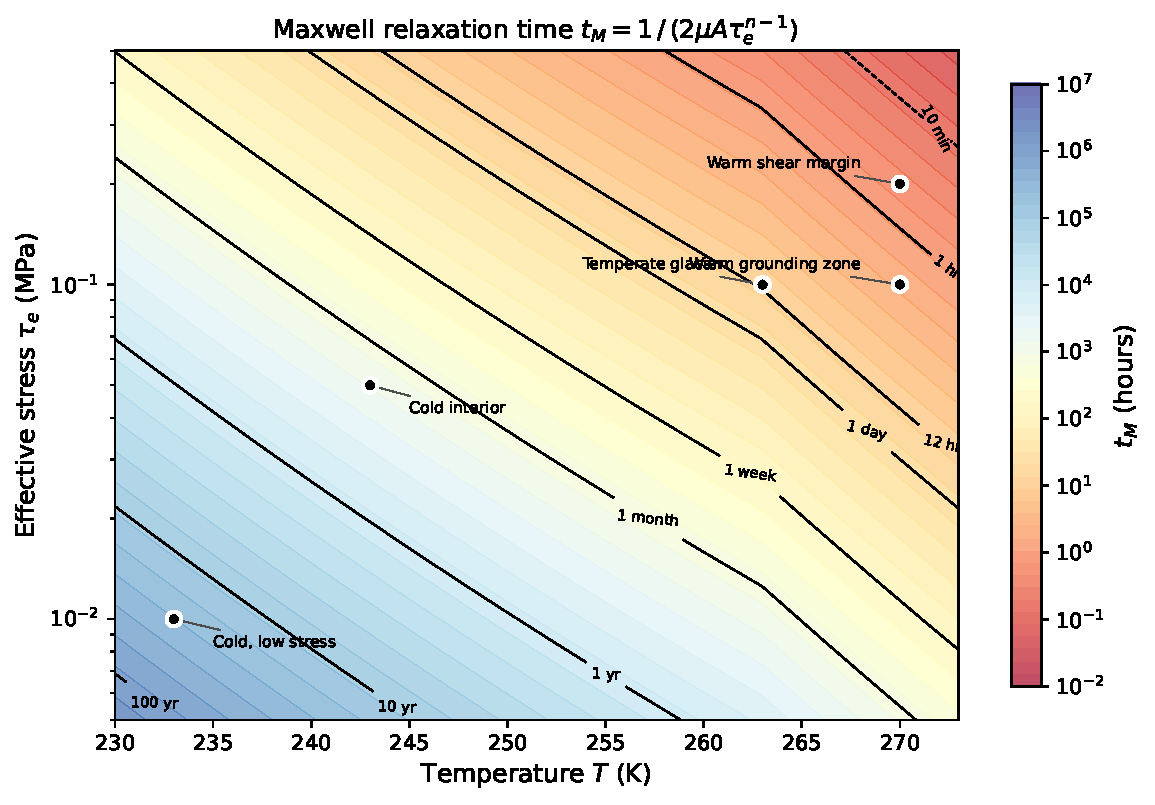
\includegraphics[width=0.85\textwidth]{figures/fig02_maxwell_time_contours.pdf}
\caption{Maxwell relaxation time $t_M = 1/(2\mu A\,\tau_e^{\,n-1})$ as a function of temperature and effective stress, computed using the Arrhenius relation for $A(T)$.  Contour labels indicate the relaxation time.  Black dots mark the five settings from Table~\ref{tab:maxwell_times}.}
\label{fig:maxwell_time_contours}
\end{figure}

\subsection{The Deborah Number}
\label{sec:deborah}

A useful dimensionless number for deciding whether a process is elastic, viscous, or viscoelastic is the \textbf{Deborah number}:
\begin{equation}
  \text{De} = \frac{t_M}{t_p},
  \label{eq:deborah}
\end{equation}
where $t_p$ is the characteristic timescale of the process or forcing.
\begin{itemize}
  \item $\text{De} \gg 1$: the relaxation time is much longer than the process timescale.  The viscous element has no time to respond, and the material behaves elastically.
  \item $\text{De} \ll 1$: the relaxation time is much shorter than the process timescale.  Elastic stresses relax away quickly, and the material behaves as a viscous fluid.
  \item $\text{De} \sim 1$: both elastic and viscous effects are important, and the full Maxwell constitutive equation must be used.
\end{itemize}

\begin{tcolorbox}[
  colback=blue!5,
  colframe=blue!50!black,
  title={\textbf{Key point: when does elasticity matter?}}
]
Elasticity matters when the Deborah number is of order unity or larger.  For glacier ice, this means:
\begin{itemize}
  \item \textbf{Tidal forcing} ($t_p \sim 12$~hours): De $\sim 0.04$--$0.9$ in warm ice near grounding zones.  Viscoelastic effects are important.
  \item \textbf{J\"{o}kulhlaup drainage} ($t_p \sim$ hours to days): De $\sim 0.05$--$5$ depending on conditions.  Both elastic and viscous responses are relevant.
  \item \textbf{Lake drainage / hydrofracture} ($t_p \sim$ minutes to hours): De $\gg 1$ everywhere.  The response is essentially elastic.
  \item \textbf{Seismic waves} ($t_p \sim 0.01$--$1$~s): De $\gg 1$ everywhere.  Purely elastic.
  \item \textbf{Seasonal flow variations} ($t_p \sim$ months): De $\ll 1$ in warm ice.  Viscous.
  \item \textbf{Ice-sheet evolution} ($t_p \sim 10^3$--$10^5$~years): De $\ll 1$.  Purely viscous.
\end{itemize}
The line between ``elastic'' and ``viscous'' behavior is not a property of the material alone---it depends on both the material state (which controls $t_M$) and the timescale of the process (which sets $t_p$).
\end{tcolorbox}

\begin{figure}[ht]
\centering
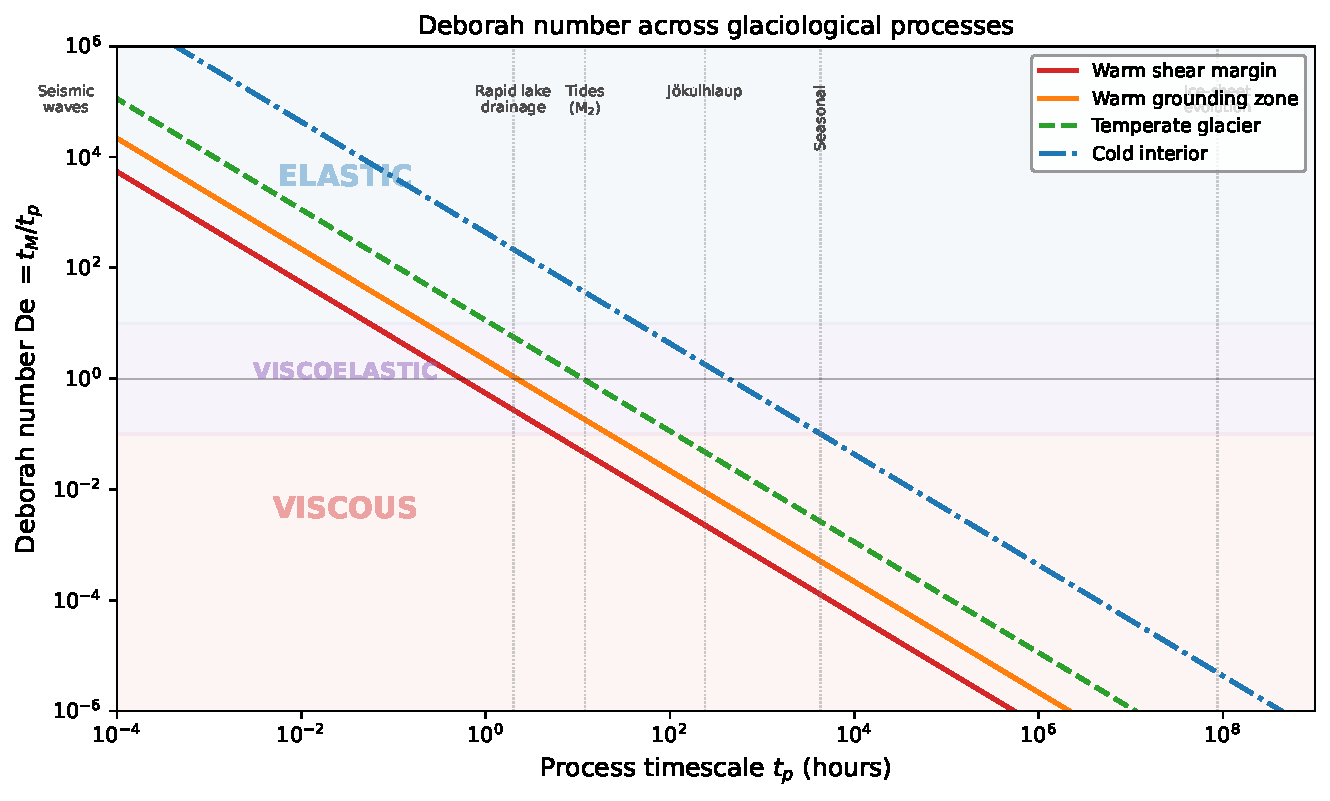
\includegraphics[width=0.95\textwidth]{figures/fig04_deborah_number.pdf}
\caption{Deborah number De~$= t_M / t_p$ as a function of process timescale for four glaciological settings (Table~\ref{tab:maxwell_times}).  Vertical dotted lines mark characteristic timescales of glaciological processes.  The shaded bands indicate the elastic ($\text{De} \gg 1$), viscoelastic ($\text{De} \sim 1$), and viscous ($\text{De} \ll 1$) regimes.}
\label{fig:deborah_number}
\end{figure}

\subsection{Response to Step Loading}
\label{sec:step_loading}

The response of a Maxwell material to an instantaneous step load reveals the interplay between elastic and viscous deformation.

\medskip
\noindent\textbf{Step stress (creep test).}  Apply a constant stress $\tau_0$ at $t = 0$.  With $\dot{\tau} = 0$ for $t > 0$, equation~\eqref{eq:maxwell_constitutive} gives:
\begin{equation}
  \varepsilon(t) = \frac{\tau_0}{2\mu} + \frac{\tau_0}{2\eta}\,t = \frac{\tau_0}{2\mu}\!\left(1 + \frac{t}{t_M}\right).
  \label{eq:creep_response}
\end{equation}
There is an instantaneous elastic strain $\tau_0/(2\mu)$ at $t = 0$, followed by a steady viscous creep at rate $\tau_0/(2\eta)$.  At $t = t_M$, the viscous strain equals the elastic strain.  For $t \gg t_M$, the elastic contribution is negligible and the response is purely viscous.

\medskip
\noindent\textbf{Step strain (relaxation test).}  Apply an instantaneous strain $\varepsilon_0$ at $t = 0$ and hold it constant ($\dot{\varepsilon} = 0$).  From equation~\eqref{eq:stress_relaxation}:
\begin{equation}
  \tau(t) = 2\mu\,\varepsilon_0\,\exp\!\left(-t/t_M\right).
  \label{eq:relaxation_response}
\end{equation}
The initial stress is $2\mu\,\varepsilon_0$ (fully elastic), and it relaxes exponentially as the viscous element accommodates the imposed strain.  After a time $t_M$, the stress has decayed to $1/e \approx 37\%$ of its initial value.  After $3\,t_M$, it has decayed to $\sim$5\%.

\medskip
\noindent\textbf{Oscillatory loading (harmonic forcing).}  For a sinusoidal stress $\tau(t) = \tau_0\,\sin(\omega t)$, the strain response of a linear Maxwell material is obtained by direct integration of the constitutive equation~\eqref{eq:maxwell_constitutive} (with $\dot{\tau} = \tau_0\,\omega\cos(\omega t)$ and $\tau/(2\eta) = \tau_0\sin(\omega t)/(2\eta)$):
\begin{equation}
  \varepsilon(t) = \frac{\tau_0}{2\mu}\,\sin(\omega t) + \frac{\tau_0}{2\eta\,\omega}\!\left[1 - \cos(\omega t)\right].
  \label{eq:harmonic_response_transient}
\end{equation}
The first term is the elastic strain (in phase with the stress); the second is the viscous contribution, which oscillates about a mean offset of $\tau_0/(2\eta\omega)$.  At high frequency ($\omega\,t_M \gg 1$), the elastic term dominates and the strain amplitude approaches $\tau_0/(2\mu)$ (elastic limit).  At low frequency ($\omega\,t_M \ll 1$), the viscous term dominates and the strain amplitude scales as $\tau_0/(\eta\omega) = \tau_0\,t_M/(\mu)$.

\medskip
\noindent The tidal flexure of ice shelves near grounding zones is a natural example of oscillatory loading.  The tidal period ($\sim$12~hours for the dominant M$_2$ constituent) is comparable to the Maxwell time of warm ice near the grounding line, placing this problem squarely in the viscoelastic regime.

\begin{figure}[ht]
\centering
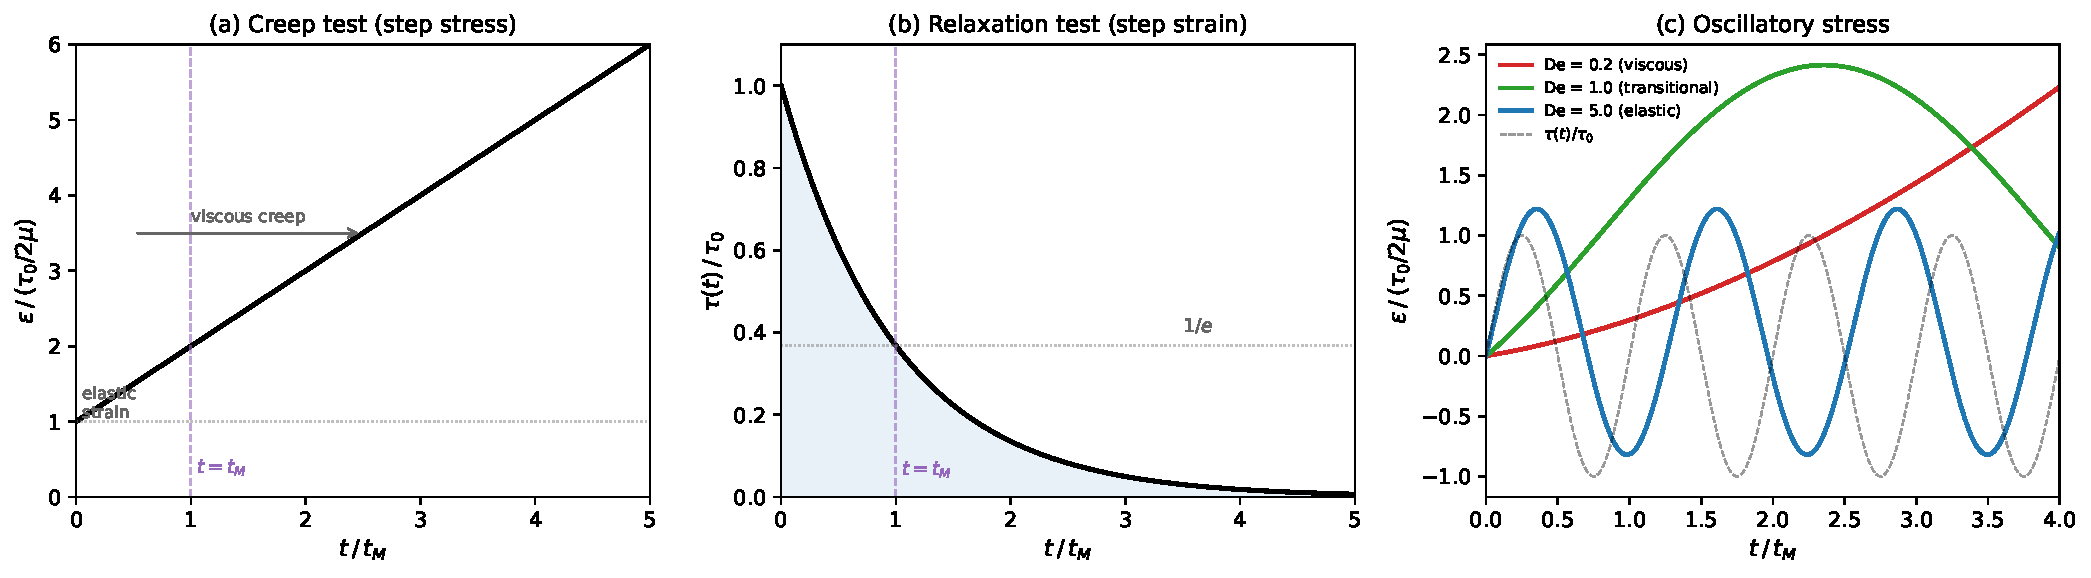
\includegraphics[width=\textwidth]{figures/fig01_maxwell_responses.pdf}
\caption{Response of a linear Maxwell material to three types of loading.  (a)~Creep test: a step stress produces an instantaneous elastic strain followed by steady viscous creep; at $t = t_M$ the viscous strain equals the elastic strain.  (b)~Relaxation test: a step strain produces an initial elastic stress that decays exponentially with $e$-folding time $t_M$.  (c)~Oscillatory stress at three Deborah numbers: for De~$= 0.2$ (viscous regime) the strain drifts; for De~$= 5$ (elastic regime) the strain oscillates in phase with the stress; for De~$= 1$ the response is transitional.}
\label{fig:maxwell_responses}
\end{figure}

%===================================================================
% SECTION 6 -- Worked Examples
%===================================================================
\section{Worked Examples}
\label{sec:worked_examples}

\subsection{Example 1: Grounding Zone Tidal Flexure}
\label{sec:example_grounding}

The grounding zone is the transition between grounded ice (resting on bedrock) and floating ice (an ice shelf or glacier tongue).  Ocean tides cause the floating ice to rise and fall, while the grounded ice remains fixed.  The transition between these two states involves flexure of the ice shelf over a horizontal distance comparable to the flexural wavelength.

\medskip
\noindent\textbf{Setup.}  Consider a one-dimensional cross section perpendicular to the grounding line.  Let $x$ denote distance from the grounding line, with $x > 0$ in the floating ice shelf and $x < 0$ in the grounded ice.  The ice shelf has uniform thickness $h$ and floats on the ocean with a tidally varying water level.  The tidal displacement at $x \to \infty$ is $w_0(t) = w_0\,\sin(\omega t)$, where $w_0$ is the tidal amplitude.  At the grounding line ($x = 0$), the ice is clamped: $w(0,t) = 0$ and $dw/dx|_{x=0} = 0$ (no deflection, no slope).

\medskip
\noindent\textbf{Elastic solution.}  The flexure equation~\eqref{eq:beam_flexure} with $q = 0$ has the general solution
\begin{equation}
  w(x) = e^{-x/\ell_f}\!\left[C_1\cos\!\left(\frac{x}{\ell_f}\right) + C_2\sin\!\left(\frac{x}{\ell_f}\right)\right] + e^{x/\ell_f}\!\left[C_3\cos\!\left(\frac{x}{\ell_f}\right) + C_4\sin\!\left(\frac{x}{\ell_f}\right)\right],
  \label{eq:flexure_general}
\end{equation}
where $\ell_f = (4D/\rho_w g)^{1/4}$.  Requiring boundedness as $x \to \infty$ sets $C_3 = C_4 = 0$.  Far from the grounding line, the ice shelf is in hydrostatic equilibrium and moves with the tide: $w(x \to \infty) = w_0$.  The solution satisfying the boundary conditions $w(0) = 0$ and $w'(0) = 0$ is
\begin{equation}
  \boxed{w(x,t) = w_0\,\sin(\omega t)\left[1 - e^{-x/\ell_f}\!\left(\cos\frac{x}{\ell_f} + \sin\frac{x}{\ell_f}\right)\right].}
  \label{eq:tidal_flexure}
\end{equation}

\begin{tcolorbox}[
  colback=orange!25,
  colframe=orange!70!black,
  title={\textbf{Derivation: tidal flexure profile}}
]
The general bounded solution for $x > 0$ is
\[
  w(x) = w_0 + e^{-x/\ell_f}\!\left[C_1\cos\frac{x}{\ell_f} + C_2\sin\frac{x}{\ell_f}\right],
\]
where we have added the far-field displacement $w_0$ as a particular solution (the weight of the tide is supported by buoyancy, not by the plate).  Applying $w(0) = 0$: $C_1 = -w_0$.  For the slope condition, write $\xi = x/\ell_f$:
\[
  w(\xi) = w_0 + e^{-\xi}\!\left[C_1\cos\xi + C_2\sin\xi\right].
\]
Differentiate:
\[
  w'(\xi) = e^{-\xi}\!\left[(-C_1 + C_2)\cos\xi + (-C_2 - C_1)\sin\xi\right].
\]
At $\xi = 0$: $w'(0) = -C_1 + C_2 = 0$, so $C_2 = C_1 = -w_0$.  Substituting:
\[
  w(x) = w_0\left[1 - e^{-x/\ell_f}\!\left(\cos\frac{x}{\ell_f} + \sin\frac{x}{\ell_f}\right)\right]. \qquad \square
\]
\end{tcolorbox}

\noindent\textbf{Bending stresses.}  The maximum bending stress occurs at the grounding line ($x = 0$), where the curvature is largest.  From equation~\eqref{eq:tidal_flexure}:
\begin{equation}
  \frac{d^2 w}{dx^2}\bigg|_{x=0} = \frac{2\,w_0}{\ell_f^2}.
  \label{eq:curvature_gl}
\end{equation}
The maximum tensile stress at the ice surface is (from equation~\eqref{eq:max_bending_stress}):
\begin{equation}
  \sigma_{\text{max}} = \frac{E\,h}{2(1-\nu^2)}\,\frac{2\,w_0}{\ell_f^2} = \frac{E\,h\,w_0}{(1-\nu^2)\,\ell_f^2}.
  \label{eq:stress_gl}
\end{equation}

\noindent\textbf{Numerical evaluation.}  For an ice shelf with $h = 500$~m and a tidal amplitude $w_0 = 1$~m:
\begin{itemize}
  \item Flexural rigidity: $D = 9.33 \times 10^9 \times 500^3 / [12 \times 0.894] = 1.09 \times 10^{17}$~N\,m.
  \item Flexural wavelength: $\ell_f = (4 \times 1.09 \times 10^{17} / (1025 \times 9.8))^{1/4} = 2.6$~km.
  \item Maximum bending stress: $\sigma_{\text{max}} = 9.33 \times 10^9 \times 500 \times 1 / (0.894 \times (2600)^2) = 770$~kPa.
\end{itemize}

\noindent This stress is below but approaching the tensile strength of ice ($\sim$1~MPa).  Tidal flexure alone does not typically fracture intact ice, but the stresses are large enough to promote fatigue crack growth in pre-existing crevasses at grounding zones, a process that has been linked to ice-shelf rifting.

\medskip
\noindent\textbf{Viscoelastic correction.}  The purely elastic solution~\eqref{eq:tidal_flexure} assumes that the ice responds instantaneously and completely to each tidal cycle.  At the grounding zone of a warm ice shelf, the Maxwell time ($t_M \sim 2$~hours; Table~\ref{tab:maxwell_times}) is comparable to the tidal period ($\sim$12~hours for M$_2$), so the Deborah number De $\approx 0.17$.  The viscous component therefore accommodates a significant fraction of the tidal flexure.  This has two consequences:
\begin{enumerate}
  \item The effective flexural rigidity is reduced, because part of the deformation is viscous and unrecoverable.  The flexural wavelength is shorter than the elastic prediction.
  \item There is a phase lag between the tidal forcing and the ice-shelf response, because the viscous element introduces a delay.
\end{enumerate}
Both effects are observed in GPS and tiltmeter measurements at Antarctic grounding zones \cite{Vaughan1995,Rignot2011}.  \cite{ElgartMinchewMeyer2026} used ICESat-2 laser altimetry to estimate the effective elastic modulus in grounding zones of the Ross Ice Shelf from tidal flexure profiles, finding that quantitative agreement with observed flexure requires accounting for viscoelastic effects through a reduced effective modulus.

\begin{figure}[ht]
\centering
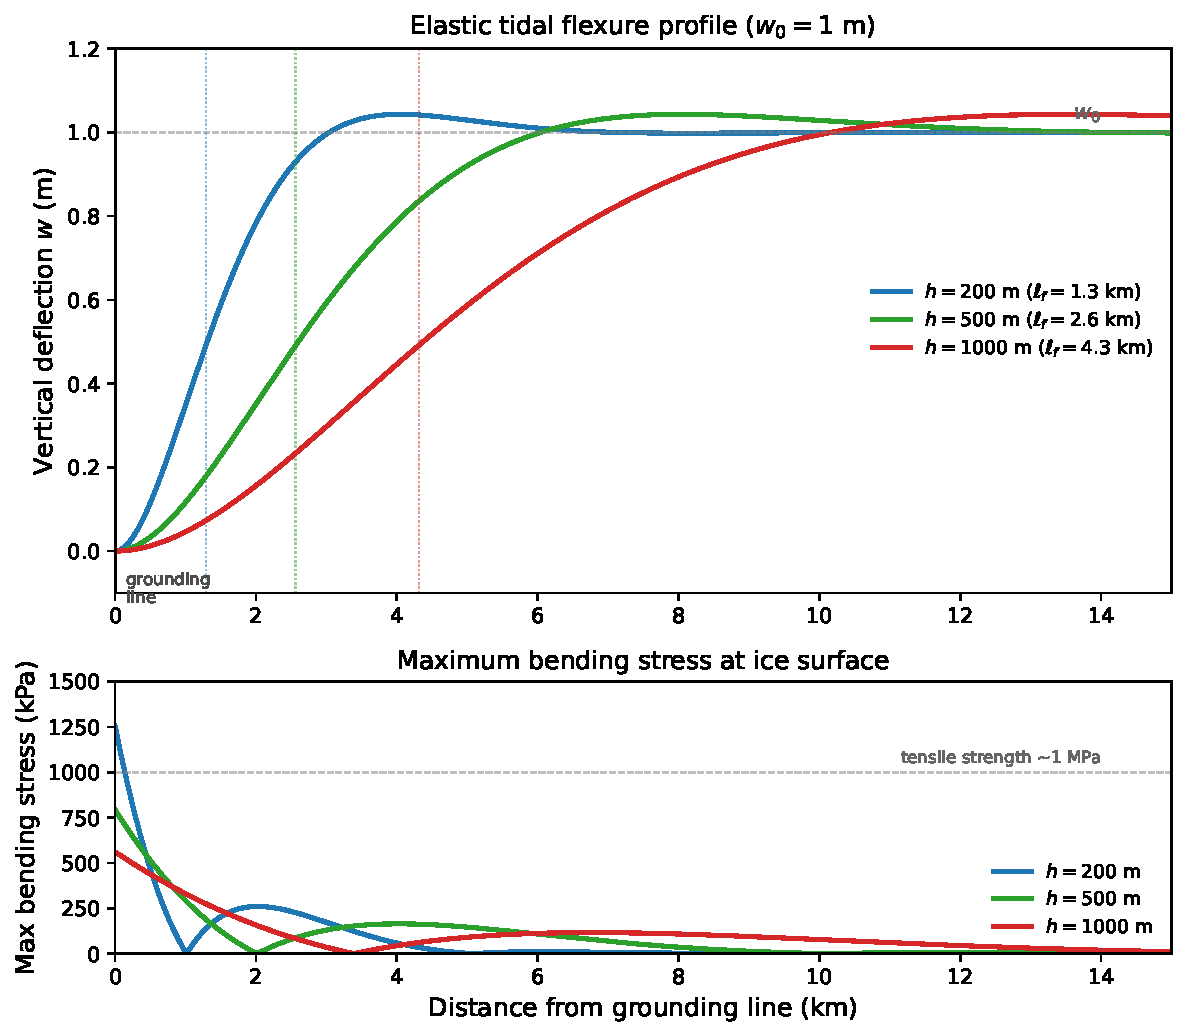
\includegraphics[width=0.85\textwidth]{figures/fig03_tidal_flexure.pdf}
\caption{Elastic tidal flexure at a grounding zone for a tidal amplitude $w_0 = 1$~m and three ice thicknesses.  Top: vertical deflection profile $w(x)$ from equation~\eqref{eq:tidal_flexure}, with the flexural wavelength $\ell_f$ marked for each thickness.  Bottom: maximum bending stress at the ice surface, showing that stresses approach but remain below the tensile strength of intact ice ($\sim$1~MPa) for thick ice shelves.}
\label{fig:tidal_flexure}
\end{figure}

\subsection{Example 2: J\"{o}kulhlaups and Elastic Rebound}
\label{sec:example_jokulhlaup}

A j\"{o}kulhlaup is a glacial outburst flood caused by the sudden drainage of a subglacial or ice-marginal lake.  The drainage removes a distributed load from the glacier surface or bed, and the ice responds to this unloading.  Whether the response is elastic, viscous, or viscoelastic depends on the drainage timescale relative to the Maxwell time.

\medskip
\noindent\textbf{Setup.}  Consider a subglacial lake of area $\mathcal{A}$ and depth $d_{\ell}$ beneath an ice sheet of thickness $h$.  The lake supports a fraction of the overburden pressure: the water pressure at the ice--lake interface is $p_w = \rho_w\,g\,d_{\ell}$.  When the lake drains on a timescale $t_d$, this hydraulic support is removed and the ice above the former lake must be supported entirely by the surrounding ice and bed.

\medskip
\noindent\textbf{Elastic limit: fast drainage.}  If $t_d \ll t_M$, the ice responds elastically.  The removal of the water load $q = \rho_w\,g\,d_{\ell}$ over the lake area produces an elastic subsidence of the ice surface.  For a circular lake of radius $R$:
\begin{itemize}
  \item If $R \ll \ell_f$: the plate is effectively rigid over the lake area, and the deflection is controlled by the plate's flexural resistance.  The maximum subsidence scales as $w \sim q\,R^4/D$.
  \item If $R \gg \ell_f$: the center of the former lake reaches isostatic equilibrium while the edges are supported by flexure.
\end{itemize}

\noindent For a more instructive estimate, consider the Deborah number.  Suppose the ice above the lake is at $T = 270$~K with $\tau_e \approx 0.1$~MPa.  From Table~\ref{tab:maxwell_times}, $t_M \approx 2$~hours.

\medskip
\noindent\textbf{Case 1: Gr\'{i}msv\"{o}tn-type j\"{o}kulhlaup} ($t_d \sim 1$--2~weeks).  The Deborah number is De $= t_M / t_d \approx 2/(24 \times 10) \approx 0.008$.  The drainage is slow compared to the Maxwell time, so the ice responds viscously.  Elastic stresses relax as the lake drains, and the surface subsidence is controlled by viscous flow.  GPS observations of surface displacement show smooth, gradual subsidence consistent with a viscous response.

\medskip
\noindent\textbf{Case 2: Rapid subglacial lake drainage} ($t_d \sim 2$~hours).  De $= t_M / t_d \approx 1.0$.  The drainage timescale is comparable to the Maxwell time.  The initial surface response is elastic---a rapid subsidence of order centimeters to decimeters---followed by viscous relaxation over subsequent hours to days.  Both elastic and viscous effects are important, and the full Maxwell model is needed to interpret surface displacement observations.

\medskip
\noindent\textbf{Elastic subsidence estimate.}  For an instantaneous drainage of a subglacial lake with $d_{\ell} = 10$~m and $R = 5$~km beneath $h = 1000$~m of ice:
\begin{equation}
  q = \rho_w\,g\,d_{\ell} = 1000 \times 9.8 \times 10 = 98 \text{ kPa},
\end{equation}
and the flexural wavelength is $\ell_f \approx 4.3$~km (for $h = 1000$~m, table in \S\ref{sec:flexure}).  Since $R \approx \ell_f$, the plate rigidity and buoyancy restoring force are both important.  The maximum elastic deflection scales as
\begin{equation}
  w_{\text{max}} \sim \frac{q\,R^4}{D} = \frac{98 \times 10^3 \times (5000)^4}{8.7 \times 10^{17}} \approx 70 \text{ m}.
  \label{eq:jokulhlaup_deflection}
\end{equation}
This crude scaling omits geometric prefactors that depend on the boundary conditions and load distribution.  For a clamped circular plate, the central deflection is $q\,R^4/(64\,D) \approx 1.1$~m; the exact value for a floating plate lies between this and the full scaling estimate.  The order of magnitude---decimeters to a meter---is consistent with GPS observations of elastic rebound following rapid subglacial lake drainage events in Antarctica \cite{Siegfriedetal2014}.

\subsection{Example 3: Supraglacial Lake Drainage and Ice-Shelf Hydrofracture}
\label{sec:example_lake}

Meltwater lakes that form on the surface of ice shelves can trigger a catastrophic chain of events: the weight of the lake water flexes the ice shelf, producing tensile stresses at the base.  If these stresses are large enough, they can initiate a fracture that propagates vertically through the full ice-shelf thickness---a process called \textbf{hydrofracture}.  Hydrofracture has been proposed as the mechanism that caused the rapid disintegration of the Larsen B Ice Shelf in 2002 \cite{ScambosHulbe2000,BanwellMacAyeal2013}.

\medskip
\noindent\textbf{Why elasticity?}  Lake loading and unloading occur on timescales of days to weeks (filling) and minutes to hours (drainage).  The Deborah number for the drainage phase is De $\gg 1$: the ice shelf responds elastically.  The elastic analysis therefore governs whether hydrofracture can initiate.

\medskip
\noindent\textbf{Setup.}  Consider a circular supraglacial lake of radius $R$ and depth $d_w$ on an ice shelf of uniform thickness $h$.  The lake applies a load $q = \rho_w\,g\,d_w$ to the ice-shelf surface (taking the lake water density as $\rho_w \approx 1000$~kg\,m$^{-3}$).  The ice shelf floats on the ocean, so the flexure equation~\eqref{eq:plate_flexure} governs the elastic deflection.

\medskip
\noindent\textbf{Flexural stress beneath the lake.}  The lake load causes the ice shelf to deflect downward beneath the lake and upward at its edges.  The downward deflection produces a concave-up curvature, which puts the bottom of the ice shelf in tension.  For a lake much smaller than the flexural wavelength ($R \ll \ell_f$), the maximum bending stress at the base of the ice shelf (at the center of the lake) scales as
\begin{equation}
  \sigma_{\text{tens}} \sim \frac{3\,(1+\nu)\,\rho_w\,g\,d_w\,R^2}{8\,h^2}.
  \label{eq:lake_stress}
\end{equation}
This is the maximum tensile stress at $z = -h/2$ beneath a uniform circular load on a thin plate, valid for $R \ll \ell_f$.  The factor $(1+\nu)$ arises from the biaxial bending moment at the center of an axisymmetric load.

\begin{tcolorbox}[
  colback=orange!25,
  colframe=orange!70!black,
  title={\textbf{Derivation: flexural stress beneath a circular lake load}}
]
For a uniform pressure $q$ over a circle of radius $R$ on an infinite plate floating on a fluid, the central deflection (for $R \ll \ell_f$) is approximately
\[
  w_0 \approx \frac{q\,R^4}{64\,D}.
\]
The curvature at the center is $\kappa = d^2w/dr^2|_{r=0} \approx q\,R^2/(16\,D)$ (from the exact Kelvin function solution in the limit $R/\ell_f \to 0$).  At the center of an axisymmetric problem, $\kappa_{rr} = \kappa_{\theta\theta} = \kappa$, so the bending stress at the bottom surface ($z = -h/2$) is
\[
  \sigma_{\text{tens}} = \frac{E\,h}{2(1-\nu^2)}\,(1+\nu)\,\kappa = \frac{E\,h\,(1+\nu)}{2(1-\nu^2)}\,\frac{q\,R^2}{16\,D} = \frac{E\,h}{2(1-\nu)}\,\frac{q\,R^2\,12(1-\nu^2)}{16\,E\,h^3} = \frac{3\,(1+\nu)\,q\,R^2}{8\,h^2}.
\]
Substituting $q = \rho_w\,g\,d_w$:
\[
  \sigma_{\text{tens}} \approx \frac{3\,(1+\nu)\,\rho_w\,g\,d_w\,R^2}{8\,h^2}. \qquad \square
\]
\end{tcolorbox}

\noindent\textbf{Numerical evaluation.}  Consider a lake with $d_w = 2$~m and $R = 500$~m on an ice shelf of thickness $h = 200$~m.  The flexural wavelength is $\ell_f \approx 1.3$~km, so $R/\ell_f \approx 0.4$ and the small-load approximation is reasonable.  Using $\nu = 0.325$:
\begin{equation}
  \sigma_{\text{tens}} \approx \frac{3 \times 1.325 \times 1000 \times 9.8 \times 2 \times 500^2}{8 \times 200^2} = \frac{1.95 \times 10^{10}}{3.2 \times 10^5} \approx 61 \text{ kPa}.
  \label{eq:lake_stress_numerical}
\end{equation}
This is about 6\% of the tensile strength of intact ice ($\sim$1~MPa).  A deeper lake ($d_w = 5$~m) or a larger lake ($R = 1$~km) would produce stresses of 150~kPa or 240~kPa, respectively---still below the tensile strength of intact ice but potentially sufficient to reactivate pre-existing crevasses, which have a much lower critical stress intensity.

\begin{figure}[ht]
\centering
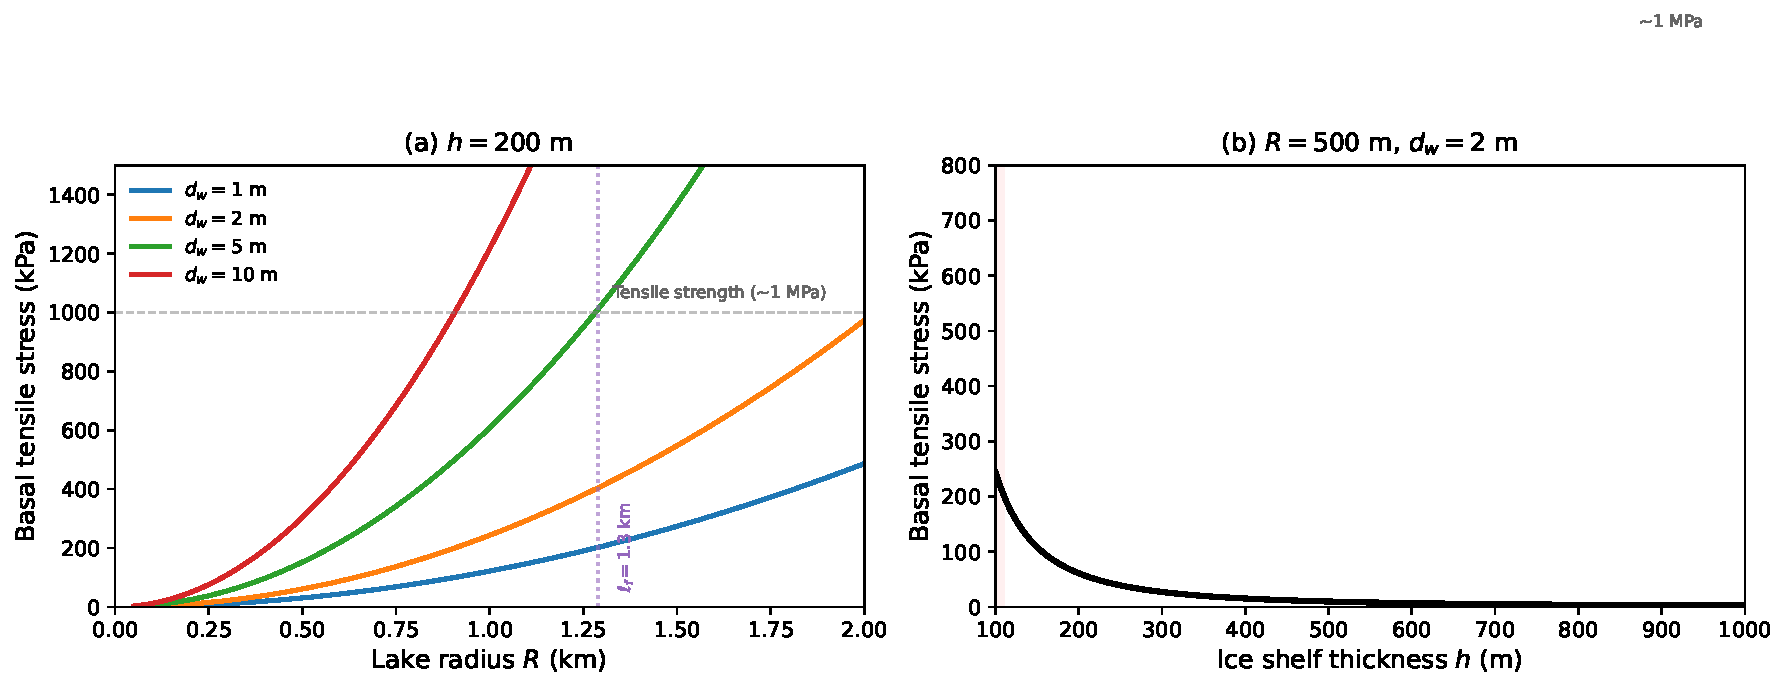
\includegraphics[width=\textwidth]{figures/fig05_lake_stress.pdf}
\caption{Basal tensile stress beneath a circular supraglacial lake from equation~\eqref{eq:lake_stress}.  (a)~Stress as a function of lake radius for several lake depths on a 200~m thick ice shelf; the flexural wavelength $\ell_f$ is marked.  (b)~Stress as a function of ice-shelf thickness for a lake with $R = 500$~m and $d_w = 2$~m, showing that thin ice shelves are most vulnerable to hydrofracture initiation.}
\label{fig:lake_stress}
\end{figure}

\medskip
\noindent\textbf{The hydrofracture feedback.}  Once a crevasse begins to propagate from the base (or surface) of the ice shelf, the water that enters the crack provides a pressure that drives the crack deeper.  The key physics is that the hydrostatic pressure of water in the crack exceeds the lithostatic (ice overburden) pressure because $\rho_w > \rho_i$: at every depth, the water pressure in a water-filled crevasse exceeds the compressive stress from the weight of the overlying ice.  This means a water-filled crevasse can, in principle, propagate through the full ice-shelf thickness regardless of thickness---a result first demonstrated by \cite{Weertman1973} and extended to ice shelves by \cite{vanderVeenCalving1998,ScambosHulbe2000}.

\medskip
\noindent The elastic flexural analysis provides the initial stress state that determines whether hydrofracture can initiate.  The subsequent propagation involves fracture mechanics (stress intensity factors, crack-tip processes) and the coupling between the fracture, the water supply, and the evolving stress field---topics beyond the scope of this lecture.

\medskip
\noindent\textbf{Connection to ice-shelf collapse.}  Prior to the disintegration of the Larsen B Ice Shelf in March 2002, satellite imagery showed extensive supraglacial lake formation on the shelf surface during the warm austral summer.  Many of these lakes drained rapidly in the days immediately preceding the collapse.  The elastic flexural stresses from the filling and draining of these lakes---compressive during filling, tensile during draining (from the elastic rebound)---are thought to have produced a ``domino effect'' in which the draining of one lake stressed neighboring regions, triggering further fracture and lake drainage \cite{BanwellMacAyeal2013}.  This example illustrates how elastic processes operating on timescales of hours to days can trigger ice-shelf disintegration events that reshape the ice-sheet system over decades.

\clearpage
%===================================================================
% Reading
%===================================================================
\section*{Reading}

Cuffey \& Paterson, \textit{Physics of Glaciers}, 4th ed.:
\begin{itemize}
  \item Section 3.2: Elasticity of ice
  \item Section 10.3: Flexure of floating ice
  \item Section 10.8: Calving and fracture
\end{itemize}

\noindent Petrenko \& Whitworth, \textit{Physics of Ice}, Chapter~4: Elastic properties.

\clearpage
%===================================================================
% APPENDIX A -- Hooke's Law from the First Law of Thermodynamics
%===================================================================
\appendix
\section{Hooke's Law from the First Law of Thermodynamics}
\label{app:hookes_law}

In this appendix, we derive Hooke's law starting from the first law of thermodynamics for a deformable body under the assumption of adiabatic conditions (no heat exchange with the surroundings).  The derivation proceeds in five steps: (1) write the first law for an adiabatic process; (2) express the rate of work done on the body in terms of surface tractions and body forces; (3) apply the divergence theorem; (4) identify Cauchy's equation of motion (the Stokes equation for a viscous fluid, or Newton's second law for a continuum) in the resulting expression; (5) define the strain energy density and deduce the form of the stiffness tensor.

\medskip
\noindent\textbf{Step 1: First law, adiabatic.}  The first law of thermodynamics states that the rate of change of total energy (internal plus kinetic) equals the rate of work done by external forces plus the rate of heat added:
\begin{equation}
  \frac{d}{dt}(U + \mathcal{K}) = \mathcal{P} + \mathcal{Q},
  \label{eq:first_law_total}
\end{equation}
where $U$ is the total internal energy, $\mathcal{K}$ is the kinetic energy, $\mathcal{P}$ is the rate of work by external forces, and $\mathcal{Q}$ is the rate of heat addition.  For an adiabatic process, $\mathcal{Q} = 0$:
\begin{equation}
  \frac{d}{dt}(U + \mathcal{K}) = \mathcal{P}.
  \label{eq:first_law_adiabatic}
\end{equation}

\noindent\textbf{Step 2: Rate of work.}  The external forces acting on a body occupying volume $V$ with surface $S$ are the surface tractions $t_i$ and body forces $f_i$ (per unit volume).  The rate of work is
\begin{equation}
  \mathcal{P} = \int_S t_i\,u_i\,dS + \int_V f_i\,u_i\,dV,
  \label{eq:power}
\end{equation}
where $u_i = \dot{s}_i$ is the velocity.

\medskip
\noindent\textbf{Step 3: Divergence theorem.}  Using Cauchy's traction formula $t_i = \sigma_{ij}\,n_j$ (where $n_j$ is the outward unit normal to $S$), the surface integral becomes
\begin{equation}
  \int_S \sigma_{ij}\,u_i\,n_j\,dS = \int_V \frac{\partial}{\partial x_j}\!\left(\sigma_{ij}\,u_i\right)dV = \int_V \left(\frac{\partial \sigma_{ij}}{\partial x_j}\,u_i + \sigma_{ij}\,\frac{\partial u_i}{\partial x_j}\right)dV,
  \label{eq:divergence}
\end{equation}
where we applied the divergence theorem in the first equality and the product rule in the second.

\medskip
\noindent\textbf{Step 4: Cauchy's equation of motion.}  Substituting~\eqref{eq:divergence} into~\eqref{eq:power}:
\begin{equation}
  \mathcal{P} = \int_V \underbrace{\left(\frac{\partial \sigma_{ij}}{\partial x_j} + f_i\right)}_{\displaystyle = \,\rho\,\dot{u}_i}\,u_i\,dV + \int_V \sigma_{ij}\,\frac{\partial u_i}{\partial x_j}\,dV.
  \label{eq:power_expanded}
\end{equation}
The bracketed term is Cauchy's equation of motion (conservation of linear momentum):
\begin{equation}
  \frac{\partial \sigma_{ij}}{\partial x_j} + f_i = \rho\,\dot{u}_i.
  \label{eq:cauchy_motion}
\end{equation}
This is the continuum form of Newton's second law.  In the Stokes equation for viscous flow, the inertial term $\rho\,\dot{u}_i$ is neglected (low Reynolds number), and the body force is gravity ($f_i = \rho\,g_i$); the form is the same.

\medskip
\noindent The first integral in~\eqref{eq:power_expanded} is the rate of change of kinetic energy:
\begin{equation}
  \int_V \rho\,\dot{u}_i\,u_i\,dV = \frac{d}{dt}\int_V \frac{1}{2}\rho\,u_i\,u_i\,dV = \frac{d\mathcal{K}}{dt}.
\end{equation}
The second integral involves $\sigma_{ij}\,\partial u_i / \partial x_j$.  Because $\sigma_{ij}$ is symmetric, only the symmetric part of $\partial u_i / \partial x_j$ contributes:
\begin{equation}
  \sigma_{ij}\,\frac{\partial u_i}{\partial x_j} = \sigma_{ij}\,\dot{\varepsilon}_{ij},
\end{equation}
where $\dot{\varepsilon}_{ij} = \frac{1}{2}(\partial u_i / \partial x_j + \partial u_j / \partial x_i)$ is the strain rate tensor.

\medskip
\noindent Substituting into the first law~\eqref{eq:first_law_adiabatic}:
\begin{equation}
  \frac{dU}{dt} = \int_V \sigma_{ij}\,\dot{\varepsilon}_{ij}\,dV.
  \label{eq:internal_energy_rate}
\end{equation}
In terms of the internal energy per unit volume $\mathcal{U}$:
\begin{equation}
  \boxed{\dot{\mathcal{U}} = \sigma_{ij}\,\dot{\varepsilon}_{ij},}
  \label{eq:strain_energy_rate}
\end{equation}
or equivalently, $d\mathcal{U} = \sigma_{ij}\,d\varepsilon_{ij}$.  All of the mechanical work done on the body (minus the kinetic energy) is stored as internal energy---strain energy---in the material.  This is the defining property of an elastic material: deformation is reversible and stores energy.

\medskip
\noindent\textbf{Step 5: Strain energy function and the stiffness tensor.}  Equation~\eqref{eq:strain_energy_rate} implies that $\mathcal{U}$ is a function of the strain: $\mathcal{U} = \mathcal{U}(\varepsilon_{ij})$, and
\begin{equation}
  \sigma_{ij} = \frac{\partial \mathcal{U}}{\partial \varepsilon_{ij}}.
  \label{eq:hyperelastic}
\end{equation}
A material for which such a strain energy function exists is called \textbf{hyperelastic}.  For small strains, expand $\mathcal{U}$ as a Taylor series about the natural (stress-free) state $\varepsilon_{ij} = 0$:
\begin{equation}
  \mathcal{U} = \underbrace{\mathcal{U}_0}_{= \,0} + \underbrace{\frac{\partial \mathcal{U}}{\partial \varepsilon_{ij}}\bigg|_0}_{= \,\sigma_{ij}|_0 \,=\, 0}\varepsilon_{ij} + \frac{1}{2}\,\underbrace{\frac{\partial^2 \mathcal{U}}{\partial \varepsilon_{ij}\,\partial \varepsilon_{kl}}\bigg|_0}_{= \,C_{ijkl}}\varepsilon_{ij}\,\varepsilon_{kl} + \cdots
  \label{eq:taylor_expansion}
\end{equation}
The zeroth-order term is the energy of the reference state (set to zero).  The first-order term vanishes because the reference state is stress-free.  The leading nontrivial term is quadratic in strain, with coefficients
\begin{equation}
  C_{ijkl} = \frac{\partial^2 \mathcal{U}}{\partial \varepsilon_{ij}\,\partial \varepsilon_{kl}}\bigg|_0.
  \label{eq:stiffness_definition}
\end{equation}
Differentiating:
\begin{equation}
  \sigma_{ij} = \frac{\partial \mathcal{U}}{\partial \varepsilon_{ij}} = C_{ijkl}\,\varepsilon_{kl}.
\end{equation}
This is Hooke's law~\eqref{eq:hookes_law_general}.  The stiffness tensor $C_{ijkl}$ inherits the major symmetry $C_{ijkl} = C_{klij}$ from the equality of mixed partial derivatives of $\mathcal{U}$---a consequence of the existence of the strain energy function, which in turn follows from the adiabatic first law.

\medskip
\noindent\textbf{Isotropic reduction.}  For an isotropic material, $C_{ijkl}$ must be invariant under all proper orthogonal transformations (rotations).  The most general isotropic fourth-order tensor with the symmetries $C_{ijkl} = C_{jikl} = C_{ijlk} = C_{klij}$ is
\begin{equation}
  C_{ijkl} = \lambda\,\delta_{ij}\,\delta_{kl} + \mu\!\left(\delta_{ik}\,\delta_{jl} + \delta_{il}\,\delta_{jk}\right),
\end{equation}
giving
\begin{equation}
  \sigma_{ij} = \lambda\,\varepsilon_{kk}\,\delta_{ij} + 2\mu\,\varepsilon_{ij},
\end{equation}
which is Hooke's law for an isotropic solid~\eqref{eq:hookes_law_isotropic}, with $\lambda$ the first Lam\'{e} parameter and $\mu$ the shear modulus.

\medskip
\noindent The strain energy density for an isotropic solid is therefore
\begin{equation}
  \mathcal{U} = \frac{1}{2}\lambda\,(\varepsilon_{kk})^2 + \mu\,\varepsilon_{ij}\,\varepsilon_{ij} = \frac{1}{2}K\,(\varepsilon_{kk})^2 + \mu\,e_{ij}\,e_{ij},
  \label{eq:strain_energy_isotropic}
\end{equation}
where the second form separates the volumetric ($K$) and deviatoric ($\mu$) contributions.  This confirms the physical interpretation: $K$ controls the energy cost of volume change, and $\mu$ controls the energy cost of shape change.

\clearpage
%===================================================================
% APPENDIX B -- The Heat Equation from the First Law
%===================================================================
\section{The Heat Equation from the First Law}
\label{app:heat_equation}

In Appendix~\ref{app:hookes_law}, we assumed adiabatic conditions ($\mathcal{Q} = 0$) and obtained the elastic constitutive relation.  Here, we take the complementary limit: allow heat flow but neglect mechanical work ($\mathcal{P} = 0$, or more precisely, neglect the strain-energy contribution).  This yields the standard heat equation.

\medskip
\noindent\textbf{First law with heat flow.}  With no mechanical work, the first law~\eqref{eq:first_law_total} reduces to
\begin{equation}
  \frac{dU}{dt} = \mathcal{Q}.
  \label{eq:first_law_heat}
\end{equation}
The rate of heat addition to a material volume $V$ has two contributions: conduction through the surface $S$ and internal heat generation at rate $H$ per unit mass:
\begin{equation}
  \mathcal{Q} = -\int_S q_i\,n_i\,dS + \int_V \rho\,H\,dV = \int_V \left(-\frac{\partial q_i}{\partial x_i} + \rho\,H\right)dV,
  \label{eq:heat_addition}
\end{equation}
where $q_i$ is the heat flux vector (positive in the direction of heat flow, hence the negative sign: heat flowing \textit{out} through the surface reduces the internal energy) and $H$ includes radiogenic heating or other volumetric sources.  We have applied the divergence theorem to convert the surface integral to a volume integral.

\medskip
\noindent Writing the internal energy per unit volume as $\mathcal{U} = \rho\,c_p\,(T - T_{\text{ref}})$ for a material with constant specific heat capacity $c_p$:
\begin{equation}
  \rho\,c_p\,\frac{\partial T}{\partial t} = -\frac{\partial q_i}{\partial x_i} + \rho\,H.
  \label{eq:energy_balance}
\end{equation}

\noindent\textbf{Fourier's law.}  The constitutive relation for heat conduction is Fourier's law:
\begin{equation}
  q_i = -k\,\frac{\partial T}{\partial x_i},
  \label{eq:fourier}
\end{equation}
where $k$ is the thermal conductivity.  For ice, $k \approx 2.1$~W\,m$^{-1}$\,K$^{-1}$ near 0\textdegree C (and increases at lower temperatures).  Substituting:
\begin{equation}
  \boxed{\rho\,c_p\,\frac{\partial T}{\partial t} = k\,\nabla^2 T + \rho\,H.}
  \label{eq:heat_equation}
\end{equation}
This is the \textbf{standard heat equation}---a parabolic partial differential equation that governs the diffusion of temperature through a material in the absence of mechanical coupling.

\medskip
\noindent The thermal diffusivity $\kappa = k / (\rho\,c_p)$ characterizes the rate of heat diffusion.  For ice ($\rho = 917$~kg\,m$^{-3}$, $c_p = 2090$~J\,kg$^{-1}$\,K$^{-1}$, $k = 2.1$~W\,m$^{-1}$\,K$^{-1}$):
\begin{equation}
  \kappa = \frac{2.1}{917 \times 2090} = 1.1 \times 10^{-6} \text{ m}^2\text{\,s}^{-1}.
\end{equation}
The characteristic diffusion time over a length scale $L$ is $t_{\text{diff}} \sim L^2 / \kappa$.  For an ice thickness of $h = 1000$~m: $t_{\text{diff}} \sim 10^{6}/(1.1 \times 10^{-6}) \approx 9 \times 10^{11}$~s~$\approx 29\,000$~years.  Temperature changes in the interior of a thick ice sheet diffuse only over timescales comparable to glacial cycles.

\clearpage
%===================================================================
% APPENDIX C -- The Generalized Heat Equation
%===================================================================
\section{The Generalized Heat Equation}
\label{app:generalized_heat}

Appendices~\ref{app:hookes_law} and~\ref{app:heat_equation} treated the two limits of the first law separately: adiabatic (no heat flow $\to$ elasticity) and no work (no deformation $\to$ heat equation).  Here we retain both terms to obtain the \textbf{generalized heat equation}, which couples mechanical dissipation to the thermal field.

\medskip
\noindent\textbf{Full first law.}  Combining the results of the previous two appendices, the internal energy balance per unit volume is
\begin{equation}
  \rho\,c_p\,\frac{\partial T}{\partial t} = \underbrace{\sigma_{ij}\,\dot{\varepsilon}_{ij}}_{\text{mechanical work}} + \underbrace{k\,\nabla^2 T}_{\text{heat conduction}} + \,\rho\,H.
  \label{eq:generalized_heat}
\end{equation}
The mechanical work term $\sigma_{ij}\,\dot{\varepsilon}_{ij}$ represents the rate at which stresses do work on the deforming material.  In the adiabatic elastic case, this work is stored as recoverable strain energy.  In a viscous fluid, this work is dissipated irreversibly as heat.

\medskip
\noindent\textbf{Viscous dissipation.}  For an incompressible viscous material ($\dot{\varepsilon}_{kk} = 0$, the condition appropriate for creeping glacier ice):
\begin{equation}
  \sigma_{ij}\,\dot{\varepsilon}_{ij} = (-p\,\delta_{ij} + \tau_{ij})\,\dot{\varepsilon}_{ij} = -p\,\dot{\varepsilon}_{kk} + \tau_{ij}\,\dot{\varepsilon}_{ij} = \tau_{ij}\,\dot{\varepsilon}_{ij} \equiv \Phi,
  \label{eq:dissipation}
\end{equation}
where $\Phi = \tau_{ij}\,\dot{\varepsilon}_{ij}$ is the \textbf{viscous dissipation function}.  Only the deviatoric stress does work; the pressure term vanishes because the flow is incompressible.  Since both $\tau_{ij}$ and $\dot{\varepsilon}_{ij}$ are related by the flow law, $\Phi$ can be written in terms of the effective stress or effective strain rate alone:
\begin{equation}
  \Phi = \tau_{ij}\,\dot{\varepsilon}_{ij} = 2\,\tau_e\,\dot{\varepsilon}_e = 2A\,\tau_e^{\,n+1},
  \label{eq:dissipation_glen}
\end{equation}
where the second equality uses $\dot{\varepsilon}_e = A\,\tau_e^n$.  The dissipation is always positive ($\Phi > 0$).

\medskip
\noindent\textbf{Energy partition and the Taylor--Quinney coefficient.}  The mechanical work $\Phi$ does not all become heat.  Some fraction is stored in the microstructure as the material deforms:
\begin{equation}
  \Phi = \Phi_{\text{heat}} + \dot{\mathcal{U}}_{\text{disl}} + \dot{\mathcal{U}}_{\text{gb}},
  \label{eq:energy_partition}
\end{equation}
where $\dot{\mathcal{U}}_{\text{disl}}$ is the rate of elastic strain energy storage due to dislocations and $\dot{\mathcal{U}}_{\text{gb}}$ is the rate of surface energy change due to recrystallization.

\medskip
\noindent \textit{Dislocation strain energy.}  Viscous creep in crystalline materials proceeds by the motion and multiplication of dislocations---line defects in the crystal lattice.  Each dislocation carries an elastic strain field, and the associated elastic energy per unit length scales as $\sim\!\mu\,b^2$, where $b$ is the magnitude of the Burgers vector ($b \approx 4.5 \times 10^{-10}$~m for basal slip in ice).  For a dislocation density $\varrho$ (total dislocation line length per unit volume), the stored elastic energy per unit volume is
\begin{equation}
  \mathcal{U}_{\text{disl}} \sim \frac{1}{2}\,\mu\,b^2\,\varrho.
  \label{eq:disl_energy}
\end{equation}
As deformation proceeds and $\varrho$ increases, energy is drawn from the mechanical work and stored in the lattice rather than converted to heat.

\medskip
\noindent \textit{Grain boundary surface energy.}  Grain boundaries carry a surface energy $\gamma_{\text{gb}}$ per unit area ($\gamma_{\text{gb}} \approx 0.065$~J\,m$^{-2}$ for ice).  If $S_V$ denotes the grain boundary area per unit volume, the stored surface energy per unit volume is
\begin{equation}
  \mathcal{U}_{\text{gb}} = \gamma_{\text{gb}}\,S_V.
  \label{eq:gb_energy}
\end{equation}
During dynamic recrystallization, new grain boundaries nucleate and existing boundaries migrate, changing $S_V$.  Nucleation of new grains increases $S_V$ and stores energy; grain growth decreases $S_V$ and releases energy as heat.

\medskip
\noindent The \textbf{Taylor--Quinney coefficient} $\beta$ is defined as the fraction of mechanical work that is converted to heat \cite{Ranganathanetal2021}:
\begin{equation}
  \Phi_{\text{heat}} = \beta\,\Phi, \qquad 0 < \beta \leq 1.
  \label{eq:taylor_quinney}
\end{equation}
The remaining fraction $(1 - \beta)\,\Phi = \dot{\mathcal{U}}_{\text{disl}} + \dot{\mathcal{U}}_{\text{gb}}$ is stored in the microstructure.

\medskip
\noindent Substituting into equation~\eqref{eq:generalized_heat}:
\begin{equation}
  \boxed{\rho\,c_p\,\frac{\partial T}{\partial t} = 2\beta\,A\,\tau_e^{\,n+1} + k\,\nabla^2 T + \rho\,H.}
  \label{eq:generalized_heat_glen}
\end{equation}
This is the \textbf{generalized heat equation for glacier ice}.  In glaciology, $\beta$ is almost universally taken to be unity: the energy stored in dislocations and grain boundaries is assumed negligible compared to the viscous dissipation.  This is a reasonable approximation for steady-state creep, where dislocation production and annihilation are in approximate balance ($\dot{\varrho} \approx 0$) and the grain size has reached a statistical steady state ($\dot{S}_V \approx 0$), so that the stored energy terms vanish.  During transient creep or active recrystallization, $\beta < 1$; measurements in metals undergoing plastic deformation give $\beta \approx 0.85$--$0.95$, though values for ice are not well constrained.  Setting $\beta = 1$, the generalized heat equation reduces to
\begin{equation}
  \rho\,c_p\,\frac{\partial T}{\partial t} = 2A\,\tau_e^{\,n+1} + k\,\nabla^2 T + \rho\,H,
  \label{eq:generalized_heat_beta1}
\end{equation}
which is the standard form used in ice-sheet models.  The temperature changes due to three effects: viscous dissipation (first term), thermal conduction (second term), and internal heat generation (third term).

\medskip
\noindent\textbf{When does viscous dissipation matter?}  The ratio of viscous heating to conductive heat transport scales as
\begin{equation}
  \frac{\Phi}{k\,\nabla^2 T} \sim \frac{2A\,\tau_e^{n+1}\,h^2}{k\,\Delta T},
\end{equation}
where $h$ is the ice thickness and $\Delta T$ is the temperature difference across it.  For typical ice-sheet conditions ($\tau_e = 0.1$~MPa, $A = 3.5 \times 10^{-25}$~Pa$^{-3}$\,s$^{-1}$ at 263~K, $h = 1000$~m, $\Delta T = 30$~K, $k = 2.1$~W\,m$^{-1}$\,K$^{-1}$):
\begin{equation}
  \frac{\Phi}{k\,\Delta T/h^2} = \frac{2 \times 3.5 \times 10^{-25} \times (10^5)^4 \times 10^6}{2.1 \times 30} = \frac{7 \times 10^{-25} \times 10^{26}}{63} = \frac{70}{63} \approx 1.1.
\end{equation}
The two terms are comparable.  Viscous dissipation is a significant heat source in the lower portions of thick, fast-flowing ice, where it warms the ice toward the pressure-melting point and softens it further---a positive feedback that concentrates deformation near the bed.  In ice streams and shear margins, where $\tau_e$ is higher and the ice is warmer, viscous dissipation can be the dominant heat source.

\medskip
\noindent\textbf{The connection between elasticity and heat.}  The first law of thermodynamics provides a unified framework for understanding both elasticity and heat conduction.  The adiabatic limit ($\mathcal{Q} = 0$) yields elasticity: mechanical work is stored reversibly as potential energy through the displacement of molecules from their equilibrium positions.  The no-work limit ($\Phi = 0$) yields the heat equation: thermal energy, associated with the random vibrational motion of molecules, diffuses through the material.  The full first law couples these two modes of energy: viscous dissipation converts ordered mechanical energy (the coherent translation and deformation of the material) into disordered thermal energy (the incoherent vibration of molecules about their lattice sites).  Elasticity and heat are two manifestations of molecular-scale energy, distinguished by whether the molecular motion is ordered (elastic, recoverable) or disordered (thermal, irreversible).

\clearpage
%===================================================================
% APPENDIX D -- Derivation of the Thin Plate Flexure Equation
%===================================================================
\section{Derivation of the Thin Plate Flexure Equation}
\label{app:flexure_derivation}

This appendix derives the governing equation for the bending of a thin elastic plate, equation~\eqref{eq:plate_flexure}, starting from the force balance on a plate element and the assumptions of Kirchhoff--Love plate theory.  The derivation proceeds in four steps: (1)~state the kinematic assumptions; (2)~compute the internal stresses and bending moments; (3)~derive the force and moment balance; (4)~combine to obtain the biharmonic equation.

\subsection*{Step 1: Kinematic assumptions}

Consider a thin plate of uniform thickness $h$, lying in the $x$--$y$ plane.  The plate's \textbf{neutral surface} (midplane) is at $z = 0$, so the plate extends from $z = -h/2$ to $z = h/2$.  The key assumptions of \textbf{Kirchhoff--Love plate theory} are:
\begin{enumerate}
  \item \textbf{Plane sections remain plane.}  Cross sections that are initially normal to the midplane remain plane and normal to the deformed midplane after bending.  This is the plate analogue of the Euler--Bernoulli beam assumption.
  \item \textbf{No through-thickness stretching.}  The plate thickness does not change during bending: $\varepsilon_{zz} = 0$.
  \item \textbf{Small deflections.}  The vertical deflection $w(x,y)$ of the midplane satisfies $|w| \ll h$ and $|\partial w/\partial x|, |\partial w/\partial y| \ll 1$, so that the geometry remains approximately flat.
\end{enumerate}

\noindent Under these assumptions, the displacement field at any point $(x,y,z)$ in the plate is determined entirely by the midplane deflection $w(x,y)$:
\begin{equation}
  s_x(x,y,z) = -z\,\frac{\partial w}{\partial x}, \qquad s_y(x,y,z) = -z\,\frac{\partial w}{\partial y}, \qquad s_z(x,y,z) = w(x,y).
  \label{eq:plate_displacement}
\end{equation}
The first two expressions state that horizontal displacements arise from the rotation of the cross section: a point at height $z$ above the midplane moves horizontally by $-z$ times the local slope.

\subsection*{Step 2: Strains, stresses, and bending moments}

The in-plane strains follow from differentiating equation~\eqref{eq:plate_displacement}:
\begin{equation}
  \varepsilon_{xx} = \frac{\partial s_x}{\partial x} = -z\,\frac{\partial^2 w}{\partial x^2}, \quad \varepsilon_{yy} = -z\,\frac{\partial^2 w}{\partial y^2}, \quad \varepsilon_{xy} = \frac{1}{2}\!\left(\frac{\partial s_x}{\partial y} + \frac{\partial s_y}{\partial x}\right) = -z\,\frac{\partial^2 w}{\partial x\,\partial y}.
  \label{eq:plate_strains}
\end{equation}
All strains are proportional to $z$: the midplane ($z = 0$) is unstrained, and the strains increase linearly toward the surfaces.  The curvatures of the midplane are $\kappa_{xx} = -\partial^2 w/\partial x^2$, $\kappa_{yy} = -\partial^2 w/\partial y^2$, and $\kappa_{xy} = -\partial^2 w/\partial x\,\partial y$, so that $\varepsilon_{ij} = z\,\kappa_{ij}$.

\medskip
\noindent For a thin plate under bending, the through-thickness normal stress $\sigma_{zz}$ is negligible compared to the in-plane stresses (this is the \textbf{plane stress} assumption: $\sigma_{zz} = 0$).  Substituting the plane-stress form of Hooke's law:
\begin{equation}
  \sigma_{xx} = \frac{E}{1-\nu^2}\!\left(\varepsilon_{xx} + \nu\,\varepsilon_{yy}\right) = -\frac{E\,z}{1-\nu^2}\!\left(\frac{\partial^2 w}{\partial x^2} + \nu\,\frac{\partial^2 w}{\partial y^2}\right),
  \label{eq:plate_sigma_xx}
\end{equation}
and similarly for $\sigma_{yy}$ and $\tau_{xy}$.  This is the bending stress formula stated in the main text, equation~\eqref{eq:bending_stress}.

\medskip
\noindent The \textbf{bending moments} per unit width are defined by integrating the stress times the moment arm $z$ through the thickness:
\begin{equation}
  M_{xx} = \int_{-h/2}^{h/2} \sigma_{xx}\,z\,dz, \qquad M_{yy} = \int_{-h/2}^{h/2} \sigma_{yy}\,z\,dz, \qquad M_{xy} = \int_{-h/2}^{h/2} \tau_{xy}\,z\,dz.
  \label{eq:moment_definition}
\end{equation}
Substituting equation~\eqref{eq:plate_sigma_xx} and using $\int_{-h/2}^{h/2} z^2\,dz = h^3/12$:
\begin{equation}
  M_{xx} = -D\!\left(\frac{\partial^2 w}{\partial x^2} + \nu\,\frac{\partial^2 w}{\partial y^2}\right), \qquad M_{yy} = -D\!\left(\frac{\partial^2 w}{\partial y^2} + \nu\,\frac{\partial^2 w}{\partial x^2}\right), \qquad M_{xy} = -D\,(1-\nu)\,\frac{\partial^2 w}{\partial x\,\partial y},
  \label{eq:bending_moments}
\end{equation}
where $D = E\,h^3/[12(1-\nu^2)]$ is the \textbf{flexural rigidity}, equation~\eqref{eq:flexural_rigidity}.  The factor $h^3/12$ arises from the second moment of area of the plate cross section; the factor $(1-\nu^2)$ arises from the plane-stress constraint (the plate is free to contract laterally, unlike a plane-strain beam).

\subsection*{Step 3: Force and moment balance}

Consider a small element of the plate with sides $dx$ and $dy$.  The element is subject to:
\begin{itemize}
  \item \textbf{Applied loads}: a distributed transverse load $q(x,y)$ (force per unit area, positive upward) on the top surface, and a buoyancy restoring force $-\rho_w\,g\,w$ per unit area on the bottom surface (for a floating plate displaced by $w$ from equilibrium).
  \item \textbf{Internal forces}: transverse shear forces $Q_x$ and $Q_y$ (force per unit length) acting on the cross-sectional faces.
  \item \textbf{Internal moments}: bending moments $M_{xx}$, $M_{yy}$ and twisting moments $M_{xy}$ acting on the faces.
\end{itemize}

\noindent The vertical force balance on the element gives:
\begin{equation}
  \frac{\partial Q_x}{\partial x} + \frac{\partial Q_y}{\partial y} + q - \rho_w\,g\,w = 0.
  \label{eq:vertical_balance}
\end{equation}

\noindent The moment balance about the $y$-axis (taking moments on the element, neglecting higher-order terms) gives:
\begin{equation}
  \frac{\partial M_{xx}}{\partial x} + \frac{\partial M_{xy}}{\partial y} = Q_x.
  \label{eq:moment_balance_x}
\end{equation}
Similarly, the moment balance about the $x$-axis gives:
\begin{equation}
  \frac{\partial M_{yy}}{\partial y} + \frac{\partial M_{xy}}{\partial x} = Q_y.
  \label{eq:moment_balance_y}
\end{equation}
These two equations express the fact that the transverse shear forces are not independent quantities---they are determined by the spatial gradients of the bending and twisting moments.

\subsection*{Step 4: The general flexure equation for spatially varying $D$}

Substitute equations~\eqref{eq:moment_balance_x} and~\eqref{eq:moment_balance_y} into the vertical force balance~\eqref{eq:vertical_balance}:
\begin{equation}
  \frac{\partial^2 M_{xx}}{\partial x^2} + 2\,\frac{\partial^2 M_{xy}}{\partial x\,\partial y} + \frac{\partial^2 M_{yy}}{\partial y^2} + q - \rho_w\,g\,w = 0.
  \label{eq:combined_balance}
\end{equation}
Now substitute the moment--curvature relations~\eqref{eq:bending_moments}.  Because the flexural rigidity $D = E\,h^3/[12(1-\nu^2)]$ depends on the local ice thickness $h(x,y)$, $D$ must remain inside the derivatives.  Computing each term with the product rule:
\begin{align}
  \frac{\partial^2 M_{xx}}{\partial x^2} &= -\frac{\partial^2}{\partial x^2}\!\left[D\!\left(\frac{\partial^2 w}{\partial x^2} + \nu\,\frac{\partial^2 w}{\partial y^2}\right)\right], \nonumber \\[4pt]
  2\,\frac{\partial^2 M_{xy}}{\partial x\,\partial y} &= -2\,\frac{\partial^2}{\partial x\,\partial y}\!\left[D\,(1-\nu)\,\frac{\partial^2 w}{\partial x\,\partial y}\right], \nonumber \\[4pt]
  \frac{\partial^2 M_{yy}}{\partial y^2} &= -\frac{\partial^2}{\partial y^2}\!\left[D\!\left(\frac{\partial^2 w}{\partial y^2} + \nu\,\frac{\partial^2 w}{\partial x^2}\right)\right].
  \label{eq:moment_derivatives}
\end{align}
Substituting into equation~\eqref{eq:combined_balance} gives the \textbf{general flexure equation for a plate with spatially varying thickness}:
\begin{equation}
  \boxed{\frac{\partial^2}{\partial x^2}\!\left[D\!\left(\frac{\partial^2 w}{\partial x^2} + \nu\,\frac{\partial^2 w}{\partial y^2}\right)\right] + 2\,\frac{\partial^2}{\partial x\,\partial y}\!\left[D\,(1-\nu)\,\frac{\partial^2 w}{\partial x\,\partial y}\right] + \frac{\partial^2}{\partial y^2}\!\left[D\!\left(\frac{\partial^2 w}{\partial y^2} + \nu\,\frac{\partial^2 w}{\partial x^2}\right)\right] + \rho_w\,g\,w = q.}
  \label{eq:plate_flexure_variable_D}
\end{equation}
This is the form that should be used for ice shelves, where the thickness $h(x,y)$---and hence $D(x,y) \propto h^3$---varies significantly over the flexural wavelength.  The cubic dependence on thickness means that a factor-of-two change in $h$ produces an eightfold change in $D$, so even moderate thickness gradients generate substantial spatial variation in rigidity.

\medskip
\noindent In one horizontal dimension (e.g., flow-line models of ice-shelf flexure), equation~\eqref{eq:plate_flexure_variable_D} simplifies to
\begin{equation}
  \frac{d^2}{dx^2}\!\left(D\,\frac{d^2 w}{dx^2}\right) + \rho_w\,g\,w = q(x),
  \label{eq:beam_flexure_variable_D}
\end{equation}
which, when expanded, contains terms involving $dD/dx$ and $d^2D/dx^2$ that couple the thickness gradient to the deflection.

\medskip
\noindent\textbf{Constant-$D$ limit.}  When $D$ is spatially uniform (constant thickness), it factors out of the derivatives in equation~\eqref{eq:plate_flexure_variable_D}.  The three second-derivative terms then combine as:
\begin{equation}
  D\!\left(\frac{\partial^4 w}{\partial x^4} + \nu\,\frac{\partial^4 w}{\partial x^2\,\partial y^2} + 2(1-\nu)\,\frac{\partial^4 w}{\partial x^2\,\partial y^2} + \frac{\partial^4 w}{\partial y^4} + \nu\,\frac{\partial^4 w}{\partial x^2\,\partial y^2}\right) = D\!\left(\frac{\partial^4 w}{\partial x^4} + 2\,\frac{\partial^4 w}{\partial x^2\,\partial y^2} + \frac{\partial^4 w}{\partial y^4}\right) = D\,\nabla^4 w,
\end{equation}
where $\nabla^4 = \nabla^2(\nabla^2)$ is the biharmonic operator.  The Poisson's ratio terms cancel: the coefficient of $\partial^4 w/(\partial x^2\,\partial y^2)$ is $\nu + 2(1-\nu) + \nu = 2$, independent of $\nu$.  The flexure equation reduces to
\begin{equation}
  \boxed{D\,\nabla^4 w + \rho_w\,g\,w = q(x,y),}
  \label{eq:plate_flexure_derived}
\end{equation}
which is equation~\eqref{eq:plate_flexure}.  This biharmonic form is the classical plate equation of Kirchhoff (1850) and Love (1888).  It is a useful approximation when the thickness varies slowly compared to the flexural wavelength ($|\nabla h / h| \ll 1/\ell_f$), but should be replaced by equation~\eqref{eq:plate_flexure_variable_D} when this condition is violated.

\subsection*{Boundary conditions}

The flexure equation is fourth-order in each spatial coordinate, so it requires two boundary conditions at each edge.  The standard boundary conditions are:

\begin{itemize}
  \item \textbf{Clamped edge} (built-in): the deflection and slope are both zero,
  \begin{equation}
    w = 0, \qquad \frac{\partial w}{\partial n} = 0,
  \end{equation}
  where $n$ is the coordinate normal to the edge.  This is the appropriate condition at a grounding line where the ice is firmly attached to the bed (as in Example~1, \S\ref{sec:example_grounding}).

  \item \textbf{Simply supported edge}: the deflection is zero but the plate is free to rotate,
  \begin{equation}
    w = 0, \qquad M_{nn} = 0,
  \end{equation}
  where $M_{nn}$ is the bending moment about the edge.  This condition sets the curvature (and hence the bending moment) to zero at the support.

  \item \textbf{Free edge}: both the bending moment and the effective transverse shear (the \textbf{Kirchhoff shear}, which combines the transverse shear force and the gradient of the twisting moment) vanish,
  \begin{equation}
    M_{nn} = 0, \qquad Q_n + \frac{\partial M_{nt}}{\partial t} = 0,
  \end{equation}
  where $t$ is the coordinate along the edge.  The second condition is Kirchhoff's boundary condition (1850): the twisting moment gradient acts as an equivalent transverse shear, so the plate edge must satisfy a combined force condition rather than separate conditions on $Q_n$ and $M_{nt}$.  This subtlety reduces the number of boundary conditions from three (which a fourth-order equation in 1D might seem to require at each end: $M$, $Q$, and $M_{nt}$) to two, consistent with the order of the equation.
\end{itemize}

\noindent For the tidal flexure problem (\S\ref{sec:example_grounding}), the boundary conditions are: clamped at the grounding line ($w = 0$, $\partial w/\partial x = 0$ at $x = 0$) and bounded as $x \to \infty$.  The boundedness condition replaces the two conditions at the far end and, together with the two clamped conditions, fully determines the solution.

%===================================================================
% Bibliography
%===================================================================
\begin{thebibliography}{99}

\bibitem{GoldsbyKohlstedt2001}
Goldsby, D.~L.\ and D.~L.\ Kohlstedt (2001).
Superplastic deformation of ice: Experimental observations.
\textit{Journal of Geophysical Research: Solid Earth}, 106(B6), 11017--11030.
\texttt{doi:10.1029/2000JB900336}

\bibitem{Gammonetal1983}
Gammon, P.~H., H.~Kiefte, and M.~J.\ Clouter (1983).
Elastic constants of ice samples by Brillouin spectroscopy.
\textit{Journal of Physical Chemistry}, 87(21), 4025--4029.
\texttt{doi:10.1021/j100244a004}

\bibitem{KohnenBentley1973}
Kohnen, H.\ and C.~R.\ Bentley (1973).
Seismic refraction and reflection measurements at ``Byrd'' Station, Antarctica.
\textit{Journal of Glaciology}, 12(64), 101--111.
\texttt{doi:10.3189/S0022143000022747}

\bibitem{Ranganathanetal2021}
Ranganathan, M., B.\ Minchew, C.~R.\ Meyer, and M.\ Pe\v{c} (2021).
Recrystallization of ice enhances the creep and vulnerability to fracture of ice shelves.
\textit{Earth and Planetary Science Letters}, 576, 117219.
\texttt{doi:10.1016/j.epsl.2021.117219}

\bibitem{Vaughan1995}
Vaughan, D.~G.\ (1995).
Tidal flexure at ice shelf margins.
\textit{Journal of Geophysical Research}, 100(B4), 6213--6224.
\texttt{doi:10.1029/94JB02467}

\bibitem{Rignot2011}
Rignot, E., J.\ Mouginot, and B.\ Scheuchl (2011).
Antarctic grounding line mapping from differential satellite radar interferometry.
\textit{Geophysical Research Letters}, 38, L10504.
\texttt{doi:10.1029/2011GL047109}

\bibitem{Siegfriedetal2014}
Siegfried, M.~R., H.~A.\ Fricker, M.\ Roberts, T.~A.\ Scambos, and S.\ Tulaczyk (2014).
A decade of West Antarctic subglacial lake interactions from combined ICESat and CryoSat-2 altimetry.
\textit{Geophysical Research Letters}, 41, 891--898.
\texttt{doi:10.1002/2013GL058616}

\bibitem{ScambosHulbe2000}
Scambos, T.~A., C.\ Hulbe, M.\ Fahnestock, and J.\ Bohlander (2000).
The link between climate warming and break-up of ice shelves in the Antarctic Peninsula.
\textit{Journal of Glaciology}, 46(154), 516--530.
\texttt{doi:10.3189/172756500781833043}

\bibitem{BanwellMacAyeal2013}
Banwell, A.~F., D.~R.\ MacAyeal, and O.~V.\ Sergienko (2013).
Breakup of the Larsen B Ice Shelf triggered by chain reaction drainage of supraglacial lakes.
\textit{Geophysical Research Letters}, 40(22), 5872--5876.
\texttt{doi:10.1002/2013GL057694}

\bibitem{ElgartMinchewMeyer2026}
Elgart, F., B.\ Minchew, and C.~R.\ Meyer (2026).
Estimating effective elasticity in grounding zones of the Ross Ice Shelf with tidal flexure from ICESat-2.
\textit{Journal of Glaciology}, 72, e23.
\texttt{doi:10.1017/jog.2026.10137}

\bibitem{Weertman1973}
Weertman, J.\ (1973).
Can a water-filled crevasse reach the bottom surface of a glacier?
\textit{IASH Publication}, 95, 139--145.
(No DOI available for this proceedings volume.)

\bibitem{vanderVeenCalving1998}
van der Veen, C.~J.\ (1998).
Fracture mechanics approach to penetration of surface crevasses on glaciers.
\textit{Cold Regions Science and Technology}, 27(1), 31--47.
\texttt{doi:10.1016/S0165-232X(97)00022-0}

\end{thebibliography}

\end{document}
